%%%%%%%%%%%%%%%%%%%%%%%%%%%%%%%%%%%%%%%%%
% Short Sectioned Assignment
% LaTeX Template
% Version 1.0 (5/5/12)
%
% This template has been downloaded from:
% http://www.LaTeXTemplates.com
%
% Original author:
% Frits Wenneker (http://www.howtotex.com)
%
% License:
% CC BY-NC-SA 3.0 (http://creativecommons.org/licenses/by-nc-sa/3.0/)
%
%%%%%%%%%%%%%%%%%%%%%%%%%%%%%%%%%%%%%%%%%

%----------------------------------------------------------------------------------------
%	PACKAGES AND OTHER DOCUMENT CONFIGURATIONS
%----------------------------------------------------------------------------------------

\documentclass[paper=a4, fontsize=10pt]{scrartcl} % A4 paper and 10pt font size
\usepackage{setspace}
\onehalfspacing
\usepackage{amsmath,amsfonts,graphicx}
\usepackage{apacite}
\usepackage{booktabs}
%\usepackage{geometry}
\usepackage[top=1.2in, left=3.8cm, bottom=1.2in, right=3.8cm]{geometry}
%\usepackage{xcolor}
\usepackage{graphicx}
\usepackage{lipsum}% Used for dummy text.

\usepackage{listings}
\usepackage{color}
\usepackage{xcolor}
\definecolor{dkgreen}{rgb}{0,0.6,0}
\definecolor{gray}{rgb}{0.5,0.5,0.5}
\definecolor{mauve}{rgb}{0.58,0,0.82}
\definecolor{titlepagecolor}{cmyk}{1,.60,0,.40}
\definecolor{namecolor}{cmyk}{1,.50,0,.10} 
\lstset{frame=tb,
     %language=Java,
     aboveskip=3mm,
     belowskip=3mm,
     showstringspaces=false,
     columns=flexible,
     basicstyle = \ttfamily\small,
     numbers=none,
     numberstyle=\tiny\color{gray},
     keywordstyle=\color{blue},
     commentstyle=\color{dkgreen},
     stringstyle=\color{mauve},
     breaklines=true,
     breakatwhitespace=true,
     tabsize=3
}

\usepackage[T1]{fontenc} % Use 8-bit encoding that has 256 glyphs
\usepackage{fourier} % Use the Adobe Utopia font for the document - comment this line to return to the LaTeX default
\usepackage[english]{babel} % English language/hyphenation
\usepackage{amsmath,amsfonts,amsthm} % Math packages
%\usepackage[a4paper, left=2.5cm, right=3cm, top=2.5cm, bottom=2.5cm]{geometry}
%\usepackage{lipsum} % Used for inserting dummy 'Lorem ipsum' text into the template

\usepackage{sectsty} % Allows customizing section commands
\allsectionsfont{\centering \normalfont\scshape} % Make all sections centered, the default font and small caps

\usepackage{fancyhdr} % Custom headers and footers
\pagestyle{fancyplain} % Makes all pages in the document conform to the custom headers and footers
\fancyhead[L]{\textsc{COMP90007 Network Analysis}}
    \fancyhead[R]{\textsc{Student Number: 955986 Username:} peiyongw}% No page header - if you want one, create it in the same way as the footers below
\fancyfoot[L]{} % Empty left footer
\fancyfoot[C]{} % Empty center footer
\fancyfoot[R]{\thepage} % Page numbering for right footer
\renewcommand{\headrulewidth}{0pt} % Remove header underlines
\renewcommand{\footrulewidth}{0pt} % Remove footer underlines
\setlength{\headheight}{13.6pt} % Customize the height of the header

\numberwithin{equation}{section} % Number equations within sections (i.e. 1.1, 1.2, 2.1, 2.2 instead of 1, 2, 3, 4)
\numberwithin{figure}{section} % Number figures within sections (i.e. 1.1, 1.2, 2.1, 2.2 instead of 1, 2, 3, 4)
\numberwithin{table}{section} % Number tables within sections (i.e. 1.1, 1.2, 2.1, 2.2 instead of 1, 2, 3, 4)

\setlength\parindent{0pt} % Removes all indentation from paragraphs - comment this line for an assignment with lots of text

%----------------------------------------------------------------------------------------
%	TITLE SECTION
%----------------------------------------------------------------------------------------

\newcommand{\horrule}[1]{\rule{\linewidth}{#1}} % Create horizontal rule command with 1 argument of height


\begin{document}
%\thispagestyle{empty}
\begin{titlepage}
    %\thispagestyle{empty}
    \newgeometry{left=7.5cm} %defines the geometry for the titlepage
    \pagecolor{titlepagecolor}
    \noindent
    %\includegraphics[width=2cm]{logo.jpg}\\[-1em]
    \color{white}
    \makebox[0pt][l]{\rule{1.3\textwidth}{1pt}}
    \par
    \noindent
    \textbf{\textsf{The University of }} \textcolor{namecolor}{\textsf{Melbourne}}
    \vfill
    \noindent
    {\textsf{COMP90007 Internet Technologies SM2, 2018}}
    \vskip\baselineskip
    \noindent
    {\huge \textsf{Network Analysis Assignment}}
    \vskip\baselineskip
    \noindent
    \textsf{Peiyong Wang}
    \vskip\baselineskip
    \noindent
    \textcolor{namecolor}{\textsf{username }}\textsf{peiyongw}
\end{titlepage}
\restoregeometry % restores the geometry
\nopagecolor% Use this to restore the color pages to white
%\include{titlepage}
%\setcounter{page}{0}
%\thispagestyle{empty}
%\newpage
\bibliographystyle{apacite}
\title{	
\normalfont \normalsize 
\textsc{The University of Melbourne } \\ [25pt] % Your university, school and/or department name(s)
\horrule{0.5pt} \\[0.4cm] % Thin top horizontal rule
\huge COMP90007 Internet Technologies SM2, 2018
Network Analysis Assignment \\ % The assignment title
\horrule{2pt} \\[0.5cm] % Thick bottom horizontal rule
}

\author{Peiyong Wang   955986} % Your name

\date{\normalsize\today} % Today's date or a custom date

\maketitle
\pagenumbering{arabic} % Print the title
%\thispagestyle{empty}
%----------------------------------------------------------------------------------------
%	PROBLEM 1
%----------------------------------------------------------------------------------------

\section{Measuring the hop count}
In this section, the traceroute command will be run in iTerm2 on a mid-2017 15 inch Macbook Pro with Mac OS 10.13.6 (17G65) High Sierra via WiFi. The traceroute command, together with pings and iperfs are in the shell script file "process.sh", which can be seen in the Appendix. Also, the output files of "process.sh" can be seen in the Appendix section as well. The python script "data\_process.py" for data processing and plotting are run in Python 3.6.6 with packages matplotlib\cite{hunter2007matplotlib}, numpy\cite{Oliphant:2007:PSC:1251563.1251830}, pandas\cite{mckinneypandas,  mckinney-proc-scipy-2010} and sklearn\cite{sklearn_api}, which are all updated to the newest version via pip.   The output of traceroute command see "hopcount" in Appendix.

\paragraph{Ans 2.1:}By typing "man traceroute" in the terminal, we can have 
the manual of the traceroute.  Also, the manual can be obtained from \cite{traceroutemanual}.

\begin{figure}[htbp!]
		\centering
		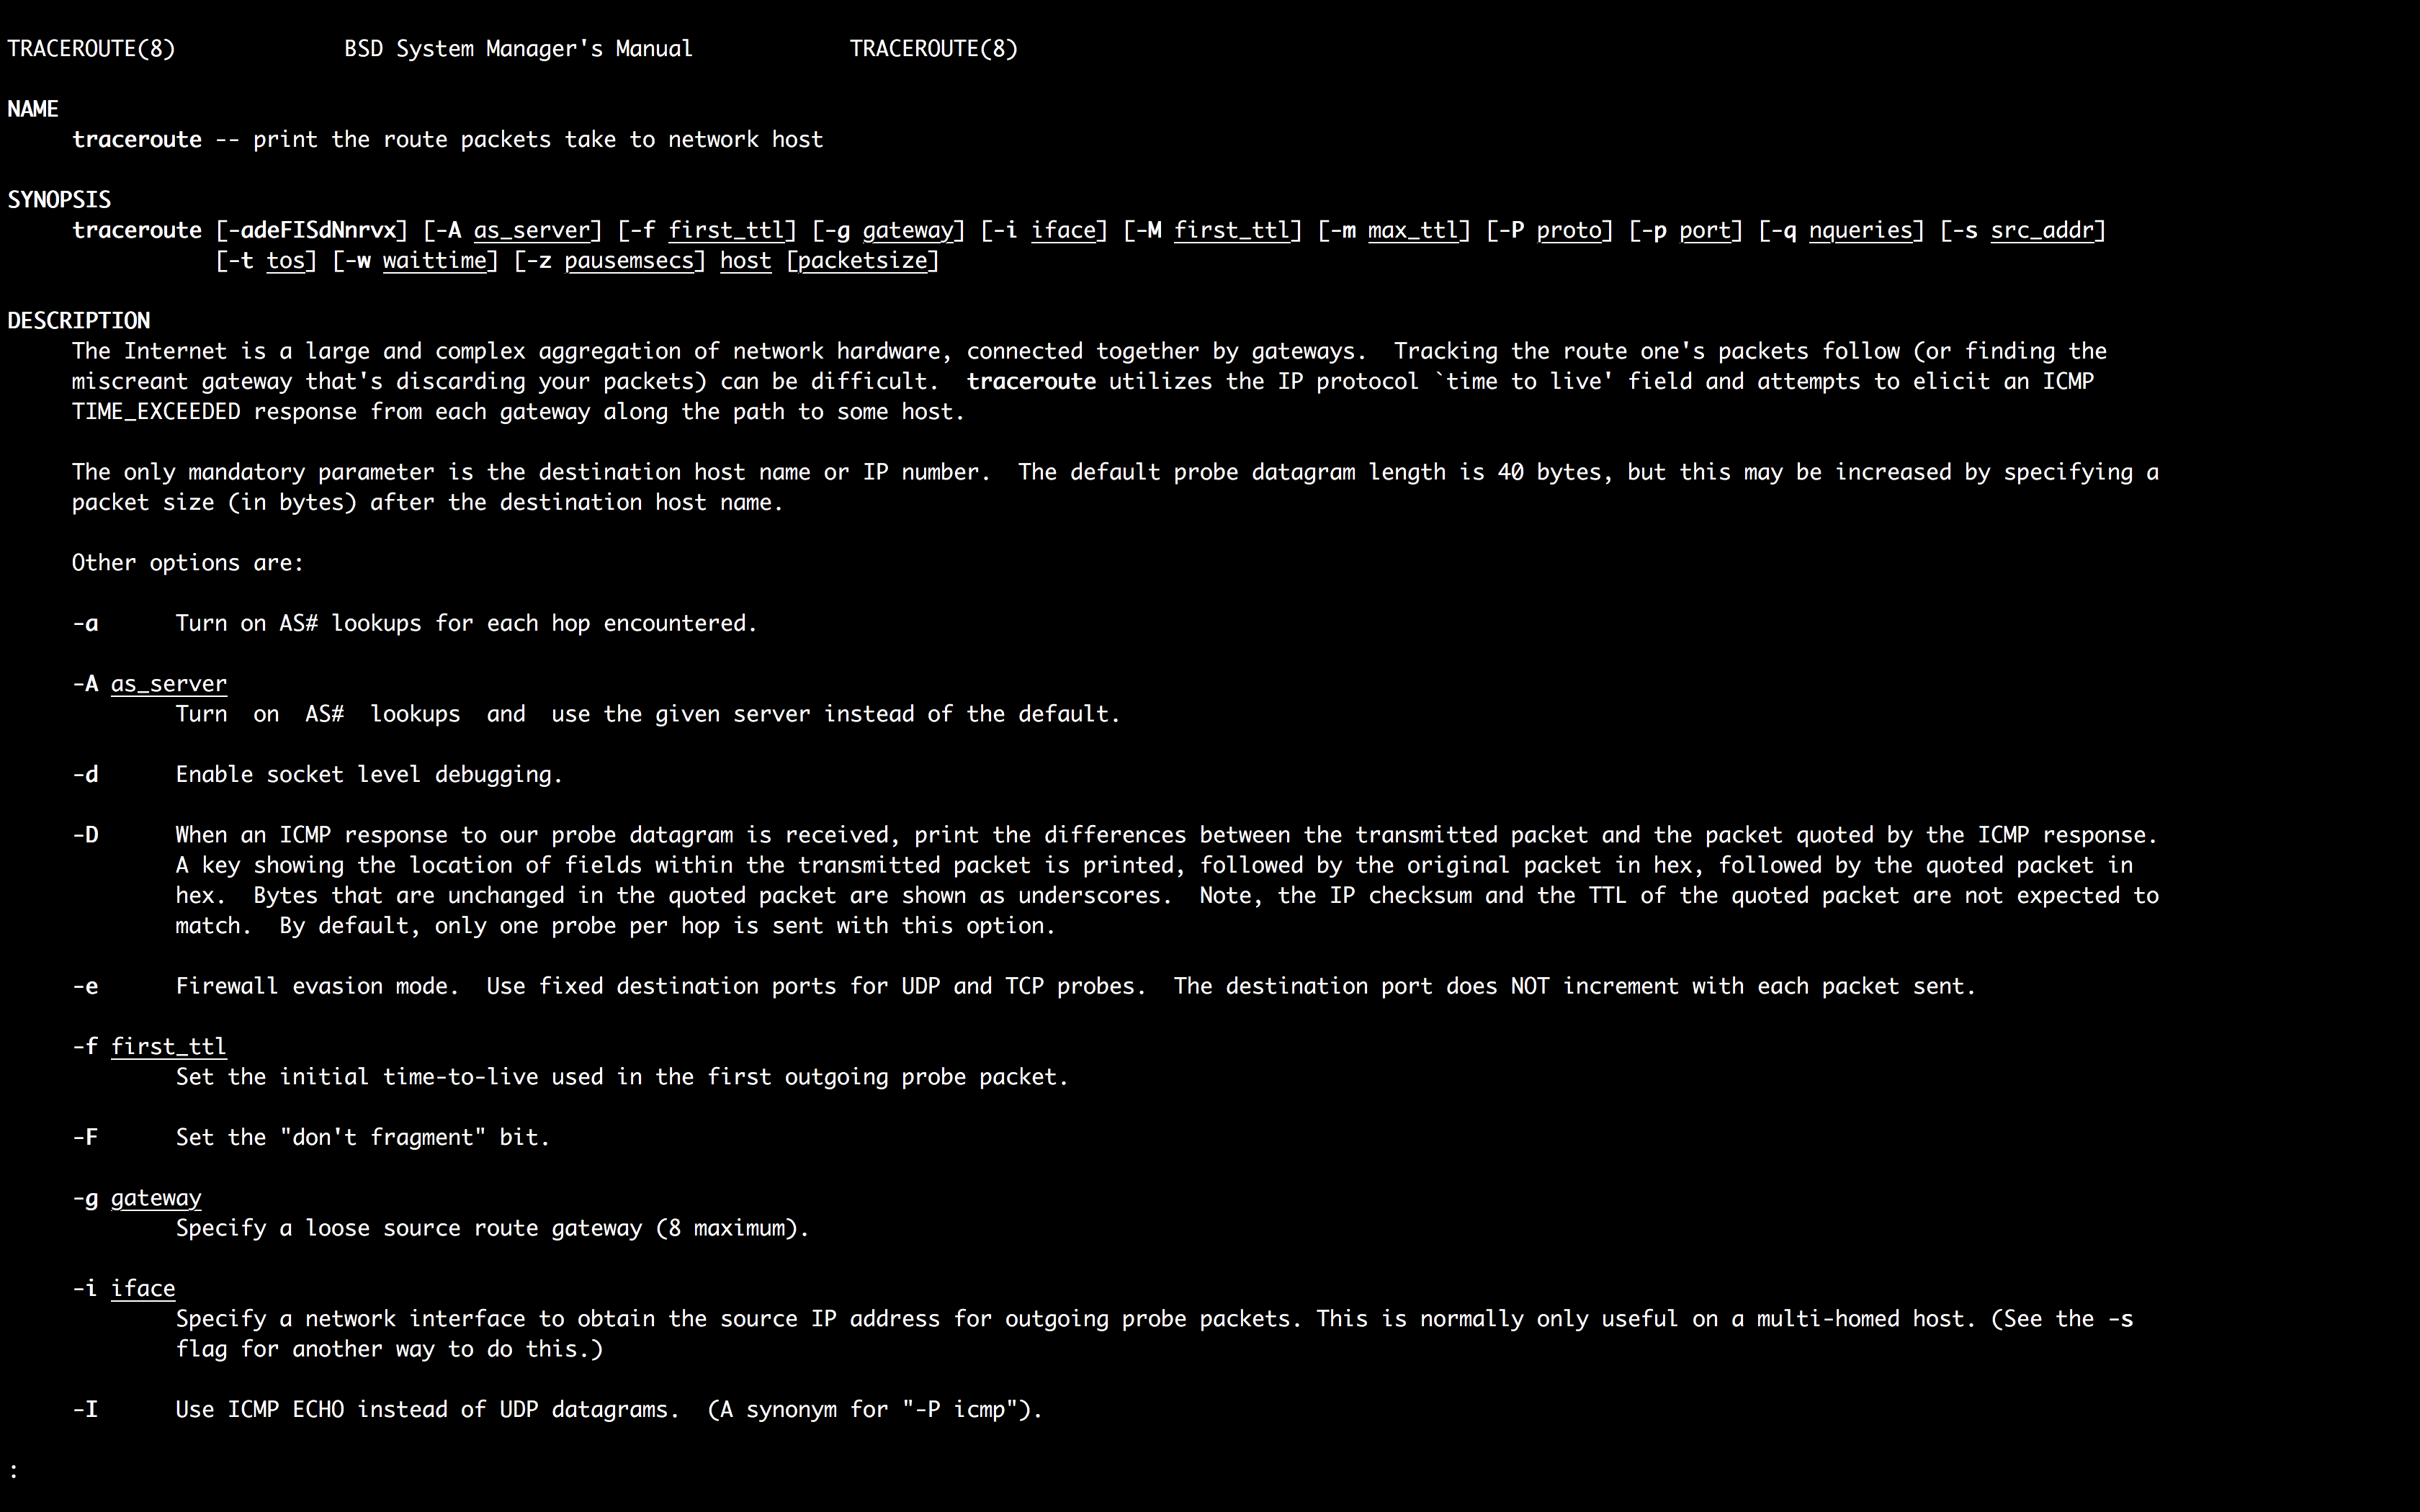
\includegraphics[width=0.6\textwidth]{fig211.png}
		\caption{Man traceroute on Mac OS High Sierra}%\label{book}
		\vspace{-1em}
\end{figure}

From the manual\cite{traceroutemanual}, we can see that the "-n" parameter is 
used to Print hop addresses numerically rather than symbolically and
numerically (saves a nameserver address-to-name lookup for each
gateway found on the path), and the "-w" parameter indicates the waiting time
for a response to a probe. In the example, the waiting time is set to 1 seconds.

For the -n parameter, by using it, the traceroute programme can only need to
print IP address numerically rather than both numerically and symbolically, which will save a nameserver address-to-name lookup for each
gateway found on the path\cite{traceroutemanual}.

For the -w 1 parameter, which sets the waiting time for just one second, and this will save a lot of time while running the traceroute programme to get the hop counts.


\paragraph{Ans 2.2}
In this assignment, we use https://www.ip-adress.com/ip-address-distance to calculate the distance between the IP address used to test traceroute, ping and iperf and Melbourne.
\begin{table}[htbp]
    \centering
    \caption{IP Addresses, Hop Counts and Distances to Melbourne}
    \begin{tabular}{ccc}
    \hline
    IP Address &Hop Count & Distance (miles) \\
    \hline
    iperf.he.net&7&7983.11\\
    bouygues.testdebit.info&19&10444.19\\
    ping.online.net&18&10481.95\\
    st2.nn.ertelecom.ru&20&8743.70\\
    iperf.biznetnetworks.com&10&3241.62\\
    ping-90ms.online.net&17&10418.95\\
    speedtest.serverius.net&19&10292.70\\
    bouygues.iperf.fr&19&10444.19\\
    iperf.volia.net&19&9193.66\\
    iperf.it-north.net&19&7585.02\\
    \hline
    \end{tabular}
\end{table}
\begin{figure}[htbp!]
    \centering
    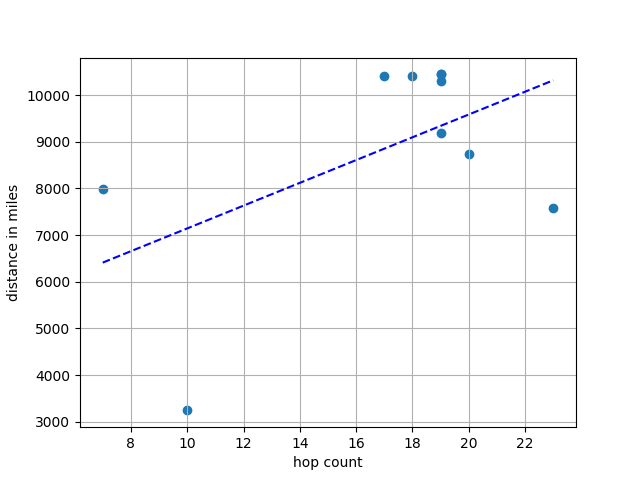
\includegraphics[width=0.6\textwidth]{hop_dist_fit.png}
    \caption{Hop Count and Distance}%\label{book}
    \vspace{-1em}
\end{figure}

We use the newest version of python package sklearn\cite{sklearn_api} to find a relationship between hop count and distance. When applying linear regression (the blue dash line in Figure 1.2), the $R^2$ of the fitting line is about 0.2734, suggesting there is a not very significant linear relationship between hop counts and distance. 

Normally, when the geographical distance between two hosts increases, the number of routers, of which common functions are routing packets and sometimes error correction, will increase. However, this assumption is not always correct. 

When the network hierarchy is very complex, or there are many layers of subnets, even the distance between the two hosts is not very long, messages traveling between these two hosts can still needed to be routed by many routers.

However, due to lack of data points, we cannot perform more complex fitting, for the data points could be over-fitted.
%\paragraph{Heading on level 4 (paragraph)}

\section{Measuring delay and jitter}
In this section, the ping command will be run in iTerm2 on a mid-2017 15 inch Macbook Pro with Mac OS 10.13.6 (17G65) High Sierra via WiFi. The performance of ping command, together with traceroute and iperfs are in the shell script file "process.sh", which can be seen in the Appendix. Also, the output files of "process.sh" can be seen in the Appendix section as well. The python script "data\_process.py" for data processing and plotting are run in Python 3.6.6 with packages matplotlib\cite{hunter2007matplotlib}, numpy\cite{Oliphant:2007:PSC:1251563.1251830}, pandas\cite{mckinneypandas,  mckinney-proc-scipy-2010} and sklearn\cite{sklearn_api}, which are all updated to the newest version via pip.   The output of this command see "pings"  in Appendix.

The data gathered in this section is listed in Table 2.1. Calculation see the python scripts in the Appendix section.
\begin{table}[htbp]
    \centering
    \caption{IP Addresses, Average Delay and Jitter}
    \begin{tabular}{ccc}
    \hline
    IP Address &Average Delay (ms) &Average Jitter (ms) \\
    \hline
    iperf.he.net&163.218&0.8129\\
    bouygues.testdebit.info&302.814&0.4577\\
    ping.online.net&301.161&0.5434\\
    st2.nn.ertelecom.ru&357.372&0.3195\\
    iperf.biznetnetworks.com&211.079&0.3858\\
    ping-90ms.online.net&389.686&0.3979\\
    speedtest.serverius.net&301.179&0.3881\\
    bouygues.iperf.fr&313.108&31.09\\
    iperf.volia.net&340.004&14.20\\
    iperf.it-north.net&395.315&2.979\\
    \hline
    \end{tabular}
\end{table}
\paragraph{Ans 3.1} When the latency is high, the user-end applications will be spending a large amount of time waiting for the responses from a distant server, so in such a circumstance the bandwidth will not be fully utilized and at the same time the performance will also decrease.

When the jitter is high, which indicates that the round-trip delay varies a lot during different time periods, the user-end application will some time runs smoothly while other time it will be spending a lot of time waiting for the packets to arrive. In such a circumstance also the bandwidth will not be fully utilized and at those high latency times the performance will be intolerable. 

Applications which require in-time data streaming, like online gaming, especially games like PUBG or DOTA2 which require swift reflexes and actions, are very sensitive to high delay and high jitter. If the connectivity decreases the game starts to lag and even stuck and the player will not be able to play games smoothly because the game starts to glitch, which will greatly affect online gaming experience.

\paragraph{Ans 3.2}
See the following figures.
\begin{figure}[htbp!]
    \centering
    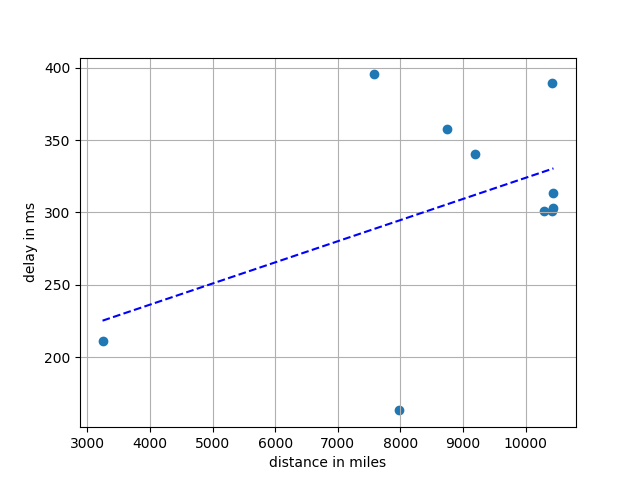
\includegraphics[width=0.6\textwidth]{dist_delay_fit.png}
    \caption{Distance and Delay}%\label{book}
    \vspace{-1em}
\end{figure}

\begin{figure}[htbp!]
    \centering
    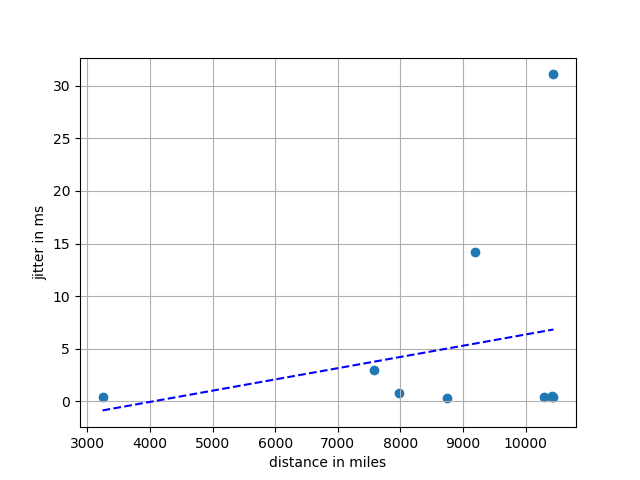
\includegraphics[width=0.6\textwidth]{distance_jitter_fit_linear.png}
    \caption{Distance and Jitter}%\label{book}
    \vspace{-1em}
\end{figure}
\newpage
\paragraph{Ans 3.3}
For delay and distance, when applying a linear regression model, the $R^2$ of the fitting function is about 0.2034. This indicates there is a not very significant linear relationship between delay and distance. As we all know, when distance increases, the time that signals need to travel from one host to another host increases. However, when the network structure is complex, the physical media needed between two hosts can be longer, which will increase the delay. In this circumstance, the routing process will also takes certain amount of time due to the complex network structure. Thus, the total delay will increase even the distance between the two hosts is not that long.

For jitter and distance, there is a very faint linear relationship between them, with a $R^2$ of about 0.05754. From Figure 2.2, we can see sometimes the jitter does not varies by distance, other time it will increase when distance increases. 

When the ping command was runing, there was no other Internet browsers active nor any download/upload tasks. Normally the download speed (via Chrome) is around 5 MB/s. So from my point of view, this faint relationship between jitter and distance is perhaps caused by different routing diagrams or pathways in the network. A sudden change in routing tables can cause a rise in jitters. Besides, I use a WiFi network which is shared by many other users living in the same apartment building as me, so there network activity may also has an impact on the delays and jitters I get from running the ping command. For example, if someone sharing the same WiFi with me is downloading some large files or watching videos, it can cause a high delay and high jitter for me.

However, without sufficient data, I can only guess the reason for the ralationships between delay and distance and jitter and distance.
\section{Measuring the bandwidth-delay product}

In this section, the iperf or iperf3 command will be run in iTerm2 on a mid-2017 15 inch Macbook Pro with Mac OS 10.13.6 (17G65) High Sierra via WiFi. The performance of iperf/iper3 command, together with traceroute and ping are in the shell script file "process.sh", which can be seen in the Appendix. Also, the output files of "process.sh" can be seen in the Appendix section as well. The python script "data\_process.py" for data processing and plotting are run in Python 3.6.6 with packages matplotlib\cite{hunter2007matplotlib}, numpy\cite{Oliphant:2007:PSC:1251563.1251830}, pandas\cite{mckinneypandas,  mckinney-proc-scipy-2010} and sklearn\cite{sklearn_api}, which are all updated to the newest version via pip.   The output of this command see "iperftest"  in Appendix.

The data gathered in this section is listed in Table 3.1. Calculation see the python scripts in the Appendix section.



\paragraph{Ans 4.1} The bandwidth-delay product determines the amount of data can be transmitted in the network. The BDP can be also viewed as the amount of data that the network can "hold" at any given time. Network with high BDP can be GEO  satellite connections, where end-to-end delivery time is high and link throughput is also high\cite{Chen:2004:UBP:2285778.2286085}.

When using a protocol which needs acknowledgement of received packets, such as TCP, if the BDP is lower than the product of the latency and available bandwidth, the network line cannot be filled since the client can't send acknowledgements back fast enough, and the throughput efficiency will be low \cite{5199079}.


\paragraph{Ans 4.2}

The data gathered is shown in Table 3.1.

\begin{table}[htbp]
    \centering
    \caption{IP Addresses, Average Bandwidth and Bandwidth-delay Product(kbp)}
    \begin{tabular}{cccc}
    \hline
    IP Address  &Average Bandwidth (kbps) &Bandwidth-delay Product\\
    \hline
    iperf.he.net&44966.66& $7.339\times 10^3 $ \\
    bouygues.testdebit.info  &20600.00& $6.238\times 10^3$ \\
    ping.online.net &17066.66& $5.140\times 10^3$\\
    st2.nn.ertelecom.ru &17466.66&$6.242\times 10^3$ \\
    iperf.biznetnetworks.com &30133.33& $6.360\times 10^3$\\
    ping-90ms.online.net &12700.00& $4.949\times 10^3$\\
    speedtest.serverius.net &19100.00& $5.752\times 10^3$\\
    bouygues.iperf.fr &16913.33& $5.296\times 10^3$\\
    iperf.volia.net &18633.33& $6.335\times 10^3$\\
    iperf.it-north.net &642.6666& $2.540\times 10^2$\\
    \hline
    \end{tabular}
\end{table} 

From Table 3.1, we can clearly see its final entry, the bandwidth and BDP for iperf.it-north.net is an outlier, which will also excluded by $2-\sigma $ bound in the following answers.
\paragraph{Ans 4.3}
\begin{figure}[htbp!]
    \centering
    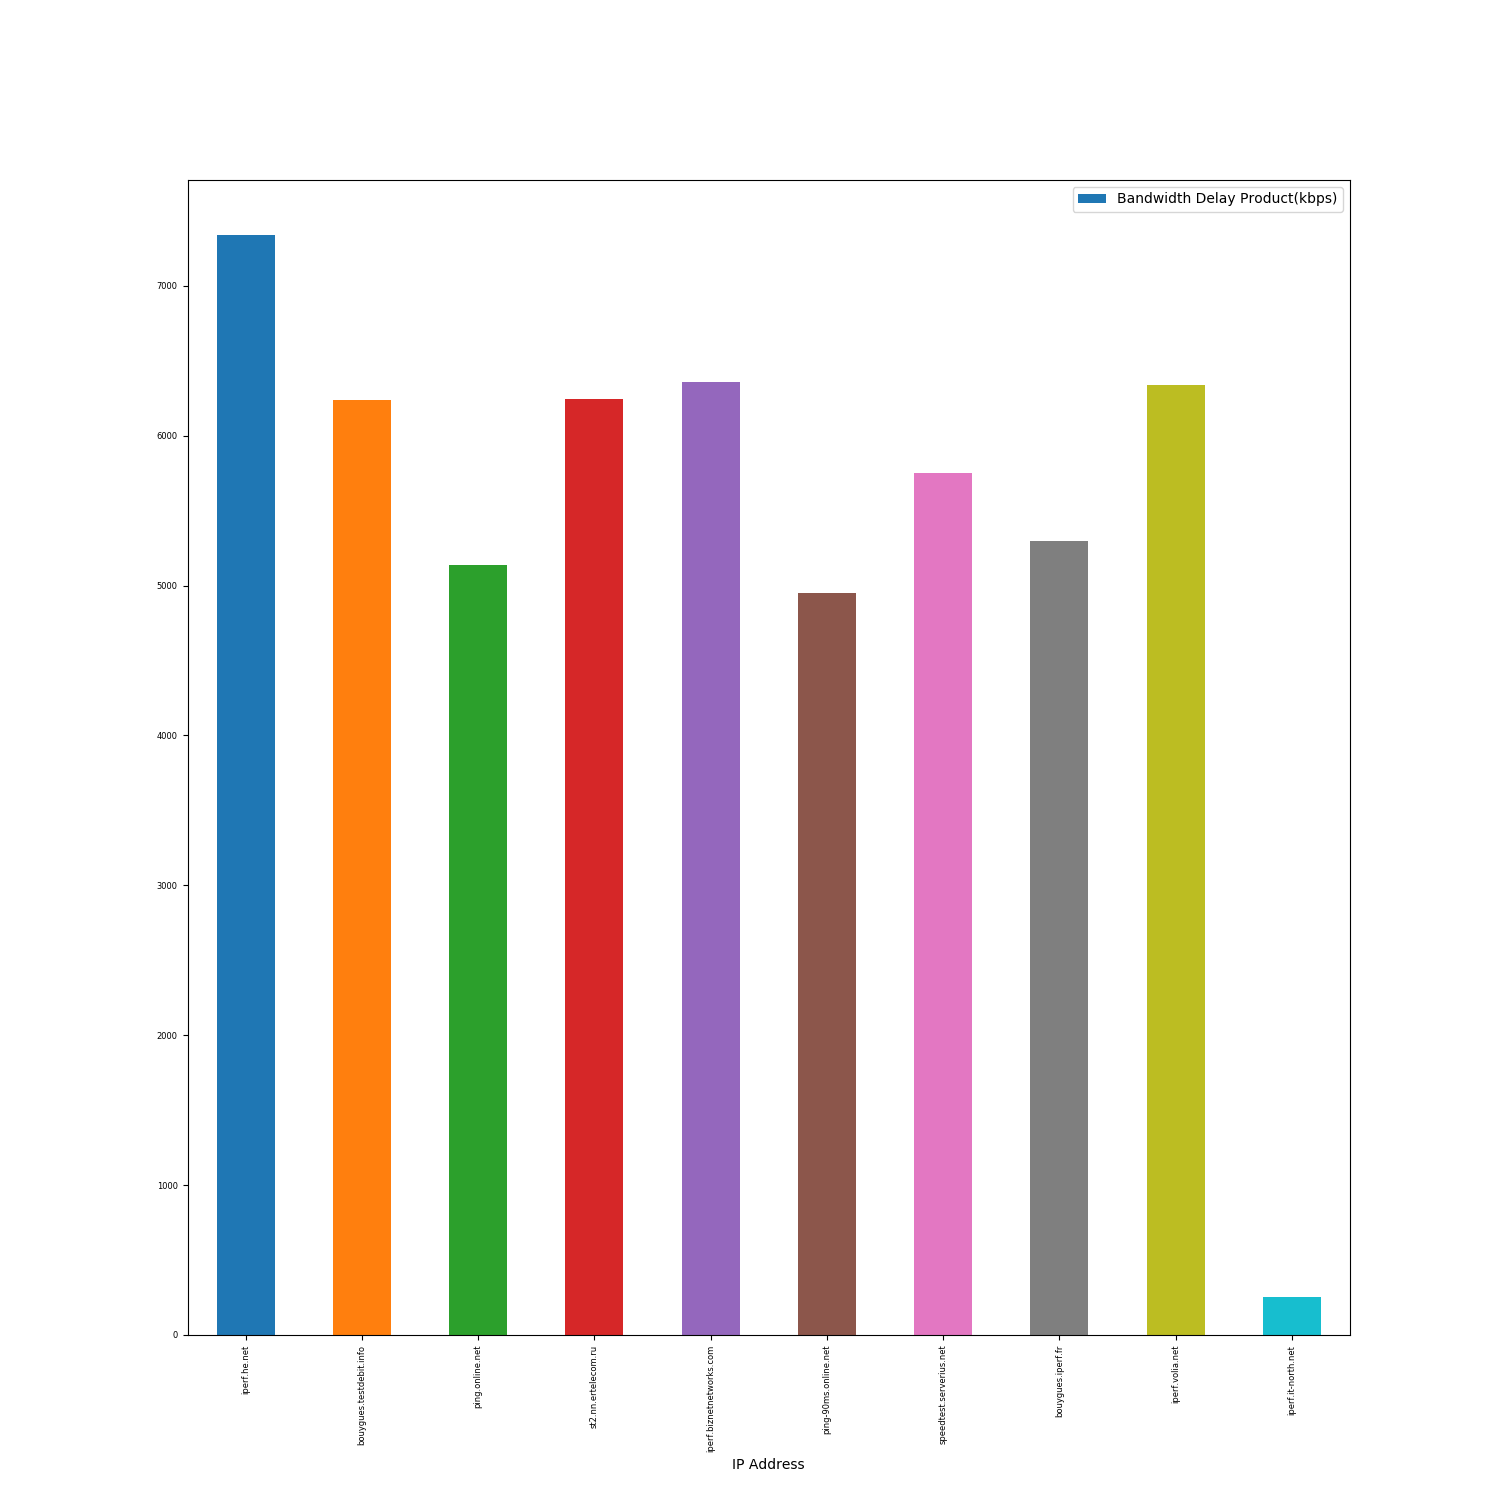
\includegraphics[width=0.99\textwidth]{bandwidth_delay_bar.png}
    \caption{Bandwidth-delay Product}%\label{book}
    \vspace{-1em}
\end{figure}
\begin{figure}[htbp!]
    \centering
    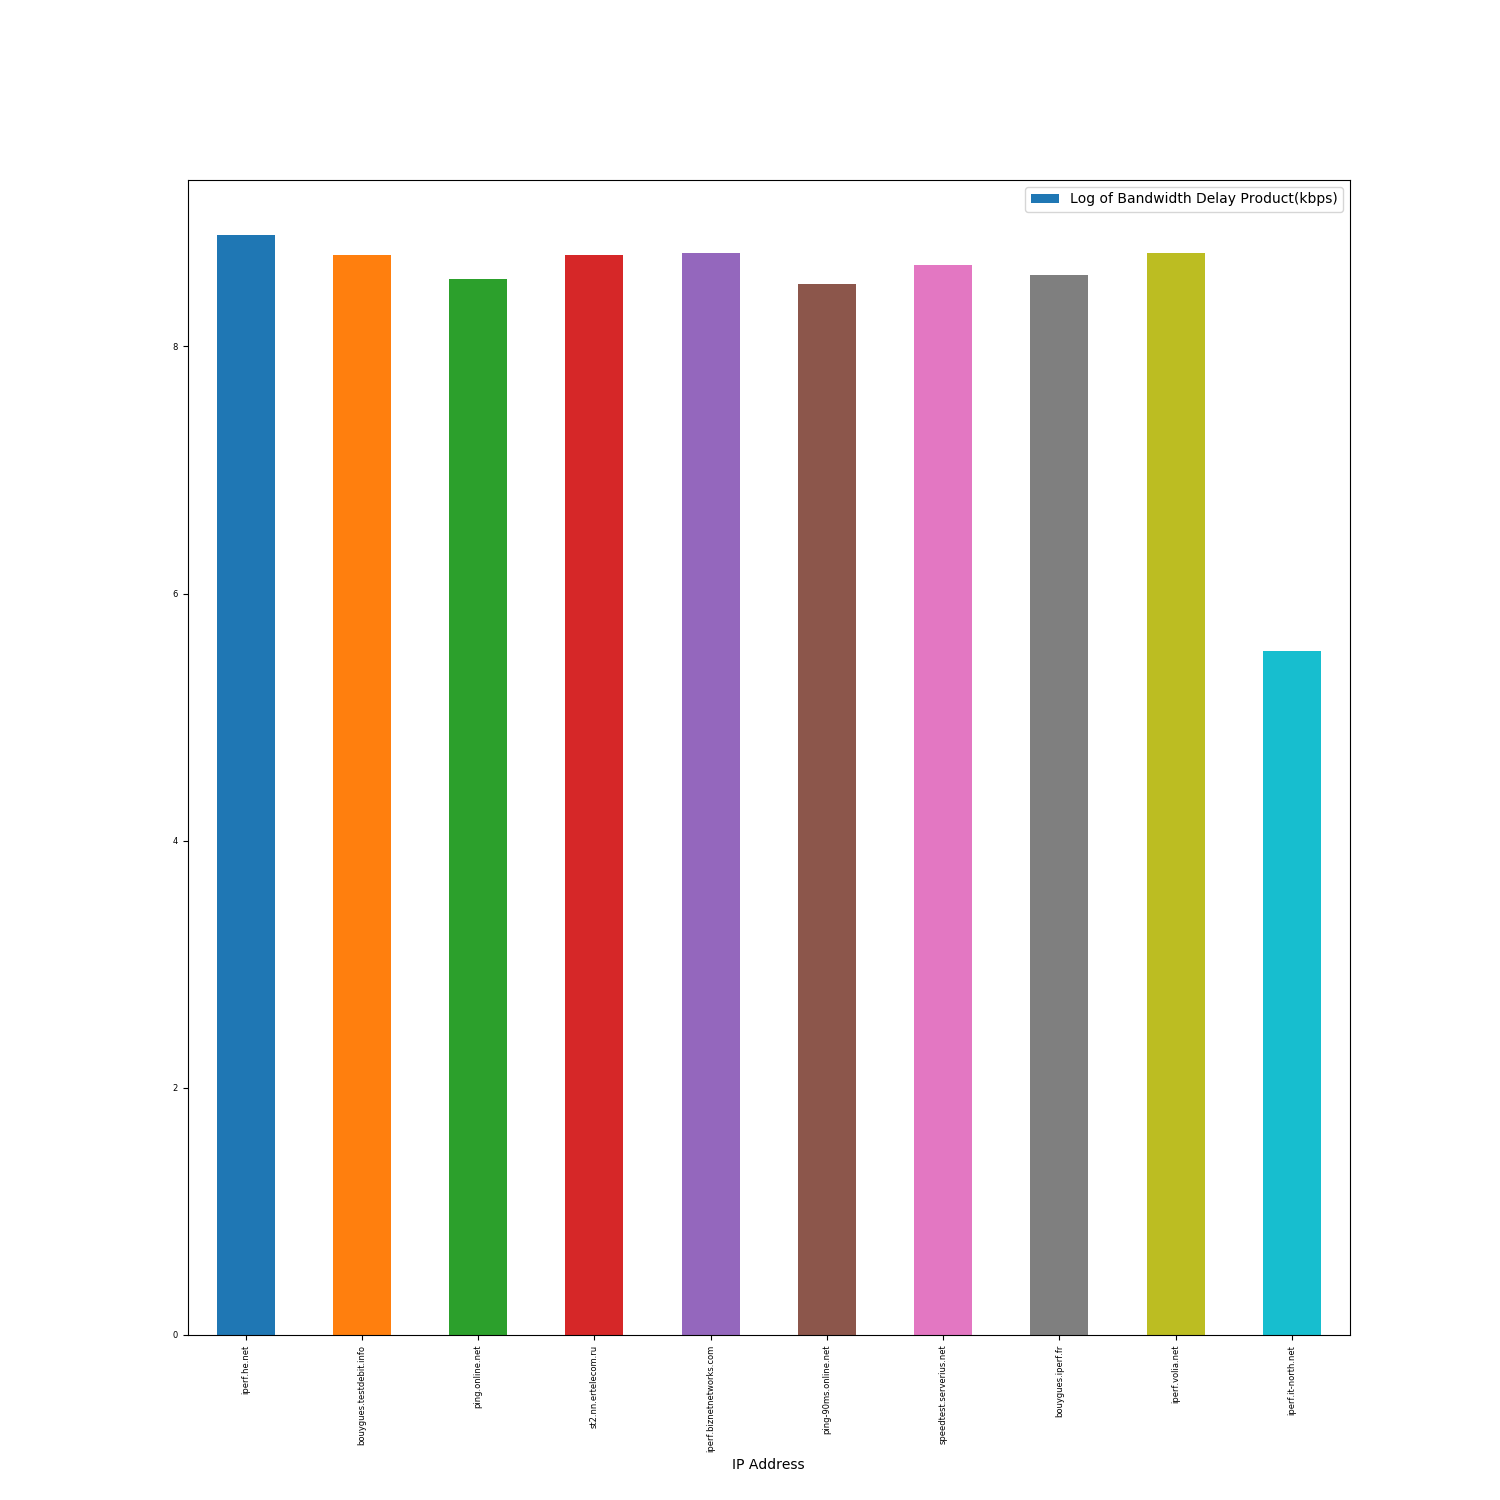
\includegraphics[width=0.99\textwidth]{bandwidth_delay_log_bar.png}
    \caption{$ln(Bandwidth-delay Product)$}%\label{book}
    \vspace{-1em}
\end{figure}

\begin{figure}[htbp!]
    \centering
    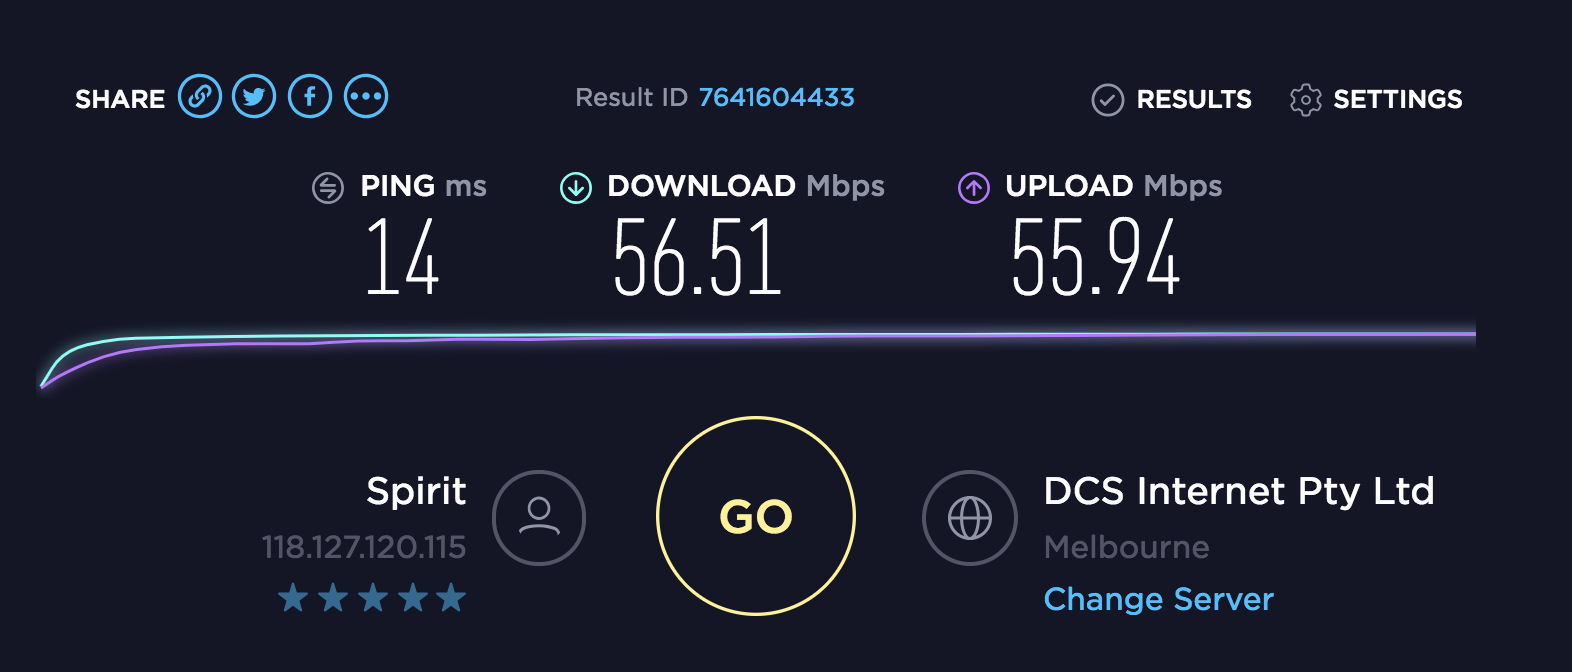
\includegraphics[width=0.99\textwidth]{43.png}
    \caption{Network Speedtest by http://eenet.speedtest.net }%\label{book}
    \vspace{-1em}
\end{figure}
As shown in the Figures 3.1 and 3.2, the BDP from iperf.it-north.net is clearly an outlier.

When the BDP is high, the actual network link speed is somehow higher (high in download and upload speed, paticularly at night, see Figure 3.3). 

From the bar charts, we can clearly see that the BDP of all hosts are pretty high except the last one (iperf.it-north.net). The average delay for this host is the biggest while the bandwidth of it is the smallest, which may indicate the conditon of the network leading to this host is not very well.

\paragraph{Ans 4.4}
See Figures 3.4 and 3.5.
\begin{figure}[htbp!]
    \centering
    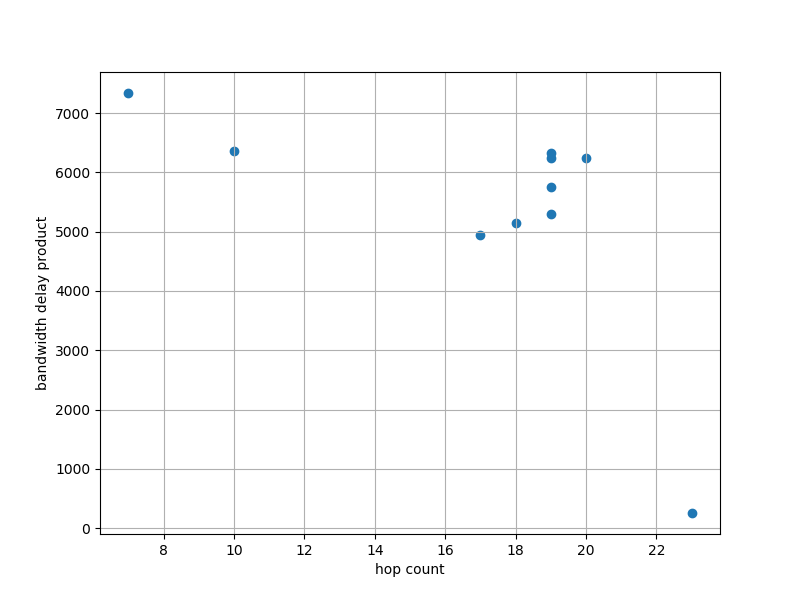
\includegraphics[width=0.99\textwidth]{hop_vs_bdp.png}
    \caption{Hop Count and BDT with Outlier, Scatter Plot}%\label{book}
    \vspace{-1em}
\end{figure}

\begin{figure}[htbp!]
    \centering
    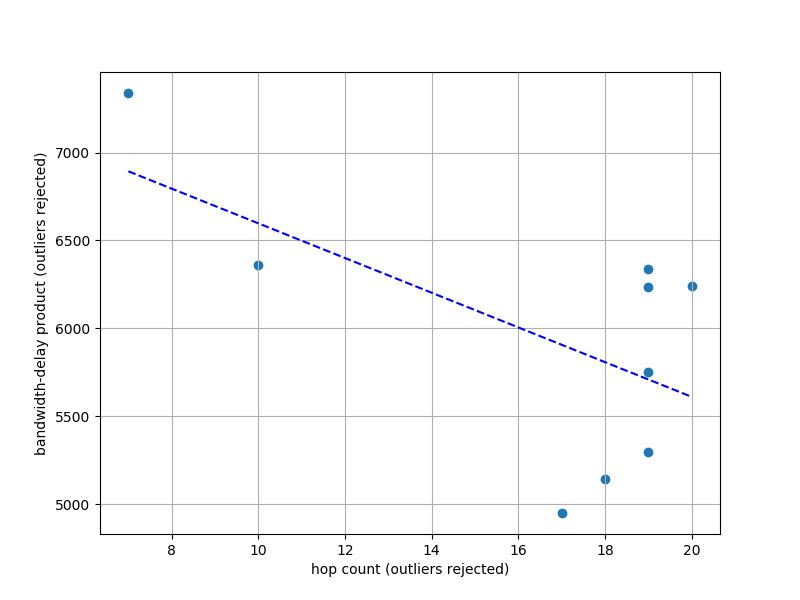
\includegraphics[width=0.99\textwidth]{hop_bdp_linear_fit_outliers_rejected.png}
    \caption{Hop Count and BDT without Outlier, Scatter Plot and Regression Line}%\label{book}
    \vspace{-1em}
\end{figure}

When rejecting the outlier(Figure 3.5), there exists a not very strong linear relationship between hop count and BDP, that the BDP drops while hop count increases, with a $ R^2$ of about 0.3697, and this relationship decays with the increase of hop count, possibly due to the changing routing condition in lang distance transmission.


\paragraph{Ans 4.5}
Due to the lack of data, all the regression results may not be accurate enough. Lack of data will easily cause over-fitting or under-fitting. And the noise of the data may be big enough to affect the results. So to improve the results one has to get sufficient amount of data (maybe thousands of data points). During the data obtaining process, I tried to excute the shell script past midnight to avoid other users in the same apartment building. And iperf/iperf3 is not always successful due to some server issues so multiple attemps was performed to get a complete set of raw data.




\newpage
\bibliography{mybib.bib}
\newpage
\section*{Appendix}
\subsection*{Appendix One: Shell script to perform all the traceroutes, pings and iperfs}
process.sh is as follows.
\begin{lstlisting}[language = bash]
    #!/bin/bash
    DATETIME="`date '+%Y%m%d%H%M%S'`" 
    
    
    cd ~/Desktop/COMP90007/network_analysis_assignment/scripts
    echo "website list
    > -----------------
    > iperf.he.net
    > bouygues.testdebit.info
    > ping.online.net
    > st2.nn.ertelecom.ru
    > iperf.biznetnetworks.com
    > ping-90ms.online.net
    > speedtest.serverius.net
    > bouygues.iperf.fr 
    > iperf.volia.net
    > iperf.it-north.net
    "
    
    [ -f iperftest ] && mv iperftest iperftest${DATETIME} || touch iperftest
    echo "Starting iperf"
    echo "Starting iperf" >> iperftest
    echo "-------------------------------------------" >> iperftest
    echo "iperf.he.net" >>iperftest
    echo "1/10"
    echo "1st">>iperftest
    iperf -c iperf.he.net >> iperftest
    echo "2nd">>iperftest
    iperf -c iperf.he.net>> iperftest
    echo "3rd">>iperftest
    iperf -c iperf.he.net>> iperftest
    echo "--------------------------------------------">>iperftest
    
    echo "bouygues.testdebit.info" >>iperftest
    echo "1st">>iperftest
    echo "2/10"
    iperf3 -c bouygues.testdebit.info -f 'm' -p 5203 >> iperftest
    echo "2nd">>iperftest
    iperf3 -c bouygues.testdebit.info -f 'm' -p 5203 >> iperftest
    echo "3rd">>iperftest
    iperf3 -c bouygues.testdebit.info -f 'm' -p 5203 >> iperftest
    echo "--------------------------------------------">>iperftest
    
    echo "ping.online.net" >>iperftest
    echo "1st">>iperftest
    echo "3/10"
    iperf3 -c ping.online.net  >> iperftest
    echo "2nd">>iperftest
    iperf3 -c ping.online.net >> iperftest
    echo "3rd">>iperftest
    iperf3 -c ping.online.net  >> iperftest
    echo "--------------------------------------------">>iperftest
    
    echo "st2.nn.ertelecom.ru" >>iperftest
    echo "4/10"
    echo "1st">>iperftest
    iperf -c st2.nn.ertelecom.ru >> iperftest
    echo "2nd">>iperftest
    iperf -c st2.nn.ertelecom.ru>> iperftest
    echo "3rd">>iperftest
    iperf -c st2.nn.ertelecom.ru>> iperftest
    echo "--------------------------------------------">>iperftest
    
    echo "iperf.biznetnetworks.com" >>iperftest
    echo "5/10"
    echo "1st">>iperftest
    iperf3 -c iperf.biznetnetworks.com -p 5202 >> iperftest
    echo "2nd">>iperftest
    iperf3 -c iperf.biznetnetworks.com -p 5202 >> iperftest
    echo "3rd">>iperftest
    iperf3 -c iperf.biznetnetworks.com -p 5202  >> iperftest
    echo "--------------------------------------------">>iperftest
    
    echo "ping-90ms.online.net" >>iperftest
    echo "6/10"
    echo "1st">>iperftest
    iperf3 -c ping-90ms.online.net  >> iperftest
    echo "2nd">>iperftest
    iperf3 -c ping-90ms.online.net  >> iperftest
    echo "3rd">>iperftest
    iperf3 -c ping-90ms.online.net  >> iperftest
    echo "--------------------------------------------">>iperftest
    
    echo "speedtest.serverius.net" >>iperftest
    echo "7/10"
    echo "1st">>iperftest
    iperf -c speedtest.serverius.net >> iperftest
    echo "2nd">>iperftest
    iperf -c speedtest.serverius.net>> iperftest
    echo "3rd">>iperftest
    iperf -c speedtest.serverius.net>> iperftest
    echo "--------------------------------------------">>iperftest
    
    echo "bouygues.iperf.fr" >>iperftest
    echo "8/10"
    echo "1st">>iperftest
    iperf3 -c bouygues.iperf.fr -f 'm'  >> iperftest
    echo "2nd">>iperftest
    iperf3 -c bouygues.iperf.fr -f 'm' >> iperftest
    echo "3rd">>iperftest
    iperf3 -c bouygues.iperf.fr -f 'm' >> iperftest
    echo " -------------------------------------------- ">>iperftest
    
    echo "iperf.volia.net" >>iperftest
    echo "9/10"
    echo "1st" >>iperftest
    iperf -c iperf.volia.net  >> iperftest
    echo "2nd" >>iperftest
    iperf -c iperf.volia.net >> iperftest
    echo "3rd" >>iperftest
    iperf -c iperf.volia.net >> iperftest
    echo "--------------------------------------------">>iperftest
    
    echo "iperf.it-north.net" >>iperftest
    echo "10/10"
    echo "1st">>iperftest
    iperf -c iperf.it-north.net  >> iperftest
    echo "2nd">>iperftest
    iperf -c iperf.it-north.net >> iperftest
    echo "3rd">>iperftest
    iperf -c iperf.it-north.net >> iperftest
    echo "--------------------------------------------">>iperftest
    
    echo "iperf ends"
    
    
    [ -f pings ] && mv pings pings${DATETIME} || touch pings
    echo "starting ping"
    echo "starting ping">>pings
    
    echo "iperf.he.net" >>pings
    echo "1/10"
    echo "1st">>pings
    ping -c 10 iperf.he.net >> pings
    echo "2nd">>pings
    ping -c 10 iperf.he.net>> pings
    echo "3rd">>pings
    ping -c 10 iperf.he.net>> pings
    echo "--------------------------------------------">>pings
    
    echo "bouygues.testdebit.info" >>pings
    echo "2/10"
    echo "1st">>pings
    ping -c 10 bouygues.testdebit.info >> pings
    echo "2nd">>pings
    ping -c 10 bouygues.testdebit.info >> pings
    echo "3rd">>pings
    ping -c 10 bouygues.testdebit.info >> pings
    echo "--------------------------------------------">>pings
    
    echo "ping.online.net" >>pings
    echo "3/10"
    echo "1st">>pings
    ping -c 10 ping.online.net >> pings
    echo "2nd">>pings
    ping -c 10 ping.online.net >> pings
    echo "3rd">>pings
    ping -c 10 ping.online.net >> pings
    echo "--------------------------------------------">>pings
    
    echo "st2.nn.ertelecom.ru" >>pings
    echo "4/10"
    echo "1st">>pings
    ping -c 10 st2.nn.ertelecom.ru >> pings
    echo "2nd">>pings
    ping -c 10 st2.nn.ertelecom.ru >> pings
    echo "3rd">>pings
    ping -c 10 st2.nn.ertelecom.ru >> pings
    echo "--------------------------------------------">>pings
    
    echo "iperf.biznetnetworks.com" >>pings
    echo "5/10"
    echo "1st">>pings
    ping -c 10 iperf.biznetnetworks.com >> pings
    echo "2nd">>pings
    ping -c 10 iperf.biznetnetworks.com >> pings
    echo "3rd">>pings
    ping -c 10 iperf.biznetnetworks.com >> pings
    echo "--------------------------------------------">>pings
    
    echo "ping-90ms.online.net" >>pings
    echo "6/10"
    echo "1st">>pings
    ping -c 10 ping-90ms.online.net >> pings
    echo "2nd">>pings
    ping -c 10 ping-90ms.online.net >> pings
    echo "3rd">>pings
    ping -c 10 ping-90ms.online.net >> pings
    echo "--------------------------------------------">>pings
    
    echo "speedtest.serverius.net" >>pings
    echo "7/10"
    echo "1st">>pings
    ping -c 10 speedtest.serverius.net >> pings
    echo "2nd">>pings
    ping -c 10 speedtest.serverius.net >> pings
    echo "3rd">>pings
    ping -c 10 speedtest.serverius.net >> pings
    echo "--------------------------------------------">>pings
    
    echo "bouygues.iperf.fr" >>pings
    echo "8/10"
    echo "1st">>pings
    ping -c 10 bouygues.iperf.fr >> pings
    echo "2nd">>pings
    ping -c 10 bouygues.iperf.fr >> pings
    echo "3rd">>pings
    ping -c 10 bouygues.iperf.fr >> pings
    echo "-------------------------------------------------"  >>pings
    
    echo "iperf.volia.net" >>pings
    echo "9/10"
    echo "1st">>pings
    ping -c 10 iperf.volia.net >> pings
    echo "2nd">>pings
    ping -c 10 iperf.volia.net >> pings
    echo "3rd">>pings
    ping -c 10 iperf.volia.net >> pings
    echo "--------------------------------------------">>pings
    
    echo "iperf.it-north.net" >>pings
    echo "10/10"
    echo "1st">>pings
    ping -c 10 iperf.it-north.net >> pings
    echo "2nd">>pings
    ping -c 10 iperf.it-north.net >> pings
    echo "3rd">>pings
    ping -c 10 iperf.it-north.net >> pings
    echo "--------------------------------------------">>pings
    
    echo "ping ends" >>pings
    echo "ping ends"
    
    [ -f hopcount ] && mv hopcount hopcount${DATETIME} || touch hopcount
    echo "Starting hopcount"
    echo "Starting hopcount" >>hopcount
    echo "--------------------------------------------">>hopcount
    echo "1/10"
    echo "iperf.he.net" >> hopcount
    traceroute -P icmp -nw1 iperf.he.net >> hopcount 
    echo "--------------------------------------------">>hopcount
    echo "2/10"
    echo "bouygues.testdebit.info" >>hopcount
    traceroute -P icmp -nw1 bouygues.testdebit.info >>hopcount
    echo "--------------------------------------------">>hopcount
    echo "3/10"
    echo "ping.online.net" >> hopcount
    traceroute -P icmp -nw1 ping.online.net >>hopcount
    echo "--------------------------------------------">>hopcount
    echo "4/10"
    echo "st2.nn.ertelecom.ru" >> hopcount
    traceroute -P icmp -nw1 st2.nn.ertelecom.ru>>hopcount
    echo "--------------------------------------------">>hopcount
    echo "5/10"
    echo "iperf.biznetnetworks.com" >> hopcount
    traceroute -P icmp -nw1 iperf.biznetnetworks.com>>hopcount
    echo "--------------------------------------------">>hopcount
    echo "6/10"
    echo "ping-90ms.online.net" >> hopcount
    traceroute -P icmp -nw1 ping-90ms.online.net>>hopcount
    echo "--------------------------------------------">>hopcount
    echo "7/10"
    echo "speedtest.serverius.net" >> hopcount
    traceroute -P icmp -nw1 speedtest.serverius.net>>hopcount
    echo "--------------------------------------------">>hopcount
    echo "8/10"
    echo "bouygues.iperf.fr" >> hopcount
    traceroute -P icmp -nw1 bouygues.iperf.fr >>hopcount
    echo "--------------------------------------------">>hopcount
    echo "9/10"
    echo "iperf.volia.net" >> hopcount
    traceroute -P icmp -nw1 iperf.volia.net >>hopcount
    echo "--------------------------------------------">>hopcount
    echo "10/10"
    echo "iperf.it-north.net" >> hopcount
    traceroute -P icmp -nw1 iperf.it-north.net >>hopcount
    echo "--------------------------------------------">>hopcount
    
    echo "hopcount completed"
    echo "hopcount completed" >> hopcount
    
    echo "ALL DONE!"
\end{lstlisting}
\subsection*{Appendix Two: Output files for the shell script}
File "iperftest"
\begin{lstlisting}
    Starting iperf
    -------------------------------------------
    iperf.he.net
    1st
    ------------------------------------------------------------
    Client connecting to iperf.he.net, TCP port 5001
    TCP window size:  129 KByte (default)
    ------------------------------------------------------------
    [  6] local 10.160.13.55 port 49960 connected with 216.218.227.10 port 5001
    [ ID] Interval       Transfer     Bandwidth
    [  6]  0.0-10.0 sec  53.6 MBytes  45.0 Mbits/sec
    2nd
    ------------------------------------------------------------
    Client connecting to iperf.he.net, TCP port 5001
    TCP window size:  129 KByte (default)
    ------------------------------------------------------------
    [  6] local 10.160.13.55 port 49966 connected with 216.218.227.10 port 5001
    [ ID] Interval       Transfer     Bandwidth
    [  6]  0.0-10.0 sec  53.6 MBytes  44.9 Mbits/sec
    3rd
    ------------------------------------------------------------
    Client connecting to iperf.he.net, TCP port 5001
    TCP window size:  129 KByte (default)
    ------------------------------------------------------------
    [  6] local 10.160.13.55 port 49972 connected with 216.218.227.10 port 5001
    [ ID] Interval       Transfer     Bandwidth
    [  6]  0.0-10.0 sec  53.8 MBytes  45.0 Mbits/sec
    --------------------------------------------
    bouygues.testdebit.info
    1st
    Connecting to host bouygues.testdebit.info, port 5203
    [  7] local 10.160.13.55 port 49982 connected to 89.84.1.222 port 5203
    [ ID] Interval           Transfer     Bitrate
    [  7]   0.00-1.00   sec   140 KBytes  1.14 Mbits/sec                  
    [  7]   1.00-2.00   sec   244 KBytes  2.00 Mbits/sec                  
    [  7]   2.00-3.00   sec  1.46 MBytes  12.3 Mbits/sec                  
    [  7]   3.00-4.00   sec  3.12 MBytes  26.3 Mbits/sec                  
    [  7]   4.00-5.00   sec  3.55 MBytes  29.8 Mbits/sec                  
    [  7]   5.00-6.00   sec  3.06 MBytes  25.6 Mbits/sec                  
    [  7]   6.00-7.00   sec  3.15 MBytes  26.4 Mbits/sec                  
    [  7]   7.00-8.00   sec  3.52 MBytes  29.5 Mbits/sec                  
    [  7]   8.00-9.01   sec  3.33 MBytes  27.8 Mbits/sec                  
    [  7]   9.01-10.00  sec  3.00 MBytes  25.1 Mbits/sec                  
    - - - - - - - - - - - - - - - - - - - - - - - - -
    [ ID] Interval           Transfer     Bitrate
    [  7]   0.00-10.00  sec  24.6 MBytes  20.6 Mbits/sec                  sender
    [  7]   0.00-10.00  sec  24.6 MBytes  20.6 Mbits/sec                  receiver
    
    iperf Done.
    2nd
    Connecting to host bouygues.testdebit.info, port 5203
    [  7] local 10.160.13.55 port 49989 connected to 89.84.1.222 port 5203
    [ ID] Interval           Transfer     Bitrate
    [  7]   0.00-1.00   sec   140 KBytes  1.15 Mbits/sec                  
    [  7]   1.00-2.00   sec   213 KBytes  1.74 Mbits/sec                  
    [  7]   2.00-3.00   sec  1.39 MBytes  11.7 Mbits/sec                  
    [  7]   3.00-4.00   sec  3.04 MBytes  25.5 Mbits/sec                  
    [  7]   4.00-5.00   sec  3.53 MBytes  29.6 Mbits/sec                  
    [  7]   5.00-6.00   sec  3.02 MBytes  25.3 Mbits/sec                  
    [  7]   6.00-7.00   sec  3.21 MBytes  27.0 Mbits/sec                  
    [  7]   7.00-8.00   sec  3.52 MBytes  29.5 Mbits/sec                  
    [  7]   8.00-9.00   sec  3.26 MBytes  27.3 Mbits/sec                  
    [  7]   9.00-10.00  sec  3.01 MBytes  25.2 Mbits/sec                  
    - - - - - - - - - - - - - - - - - - - - - - - - -
    [ ID] Interval           Transfer     Bitrate
    [  7]   0.00-10.00  sec  24.3 MBytes  20.4 Mbits/sec                  sender
    [  7]   0.00-10.00  sec  24.3 MBytes  20.4 Mbits/sec                  receiver
    
    iperf Done.
    3rd
    Connecting to host bouygues.testdebit.info, port 5203
    [  7] local 10.160.13.55 port 49996 connected to 89.84.1.222 port 5203
    [ ID] Interval           Transfer     Bitrate
    [  7]   0.00-1.00   sec   141 KBytes  1.16 Mbits/sec                  
    [  7]   1.00-2.00   sec   251 KBytes  2.06 Mbits/sec                  
    [  7]   2.00-3.00   sec  1.51 MBytes  12.7 Mbits/sec                  
    [  7]   3.00-4.00   sec  3.27 MBytes  27.5 Mbits/sec                  
    [  7]   4.00-5.00   sec  3.46 MBytes  28.9 Mbits/sec                  
    [  7]   5.00-6.00   sec  3.08 MBytes  25.8 Mbits/sec                  
    [  7]   6.00-7.00   sec  3.21 MBytes  27.1 Mbits/sec                  
    [  7]   7.00-8.00   sec  3.53 MBytes  29.6 Mbits/sec                  
    [  7]   8.00-9.00   sec  3.21 MBytes  27.0 Mbits/sec                  
    [  7]   9.00-10.00  sec  3.16 MBytes  26.5 Mbits/sec                  
    - - - - - - - - - - - - - - - - - - - - - - - - -
    [ ID] Interval           Transfer     Bitrate
    [  7]   0.00-10.00  sec  24.8 MBytes  20.8 Mbits/sec                  sender
    [  7]   0.00-10.00  sec  24.8 MBytes  20.8 Mbits/sec                  receiver
    
    iperf Done.
    --------------------------------------------
    ping.online.net
    1st
    Connecting to host ping.online.net, port 5201
    [  7] local 10.160.13.55 port 50076 connected to 62.210.18.40 port 5201
    [ ID] Interval           Transfer     Bitrate
    [  7]   0.00-1.00   sec   141 KBytes  1.16 Mbits/sec
    [  7]   1.00-2.00   sec   106 KBytes   863 Kbits/sec
    [  7]   2.00-3.00   sec   558 KBytes  4.58 Mbits/sec
    [  7]   3.00-4.00   sec  2.30 MBytes  19.3 Mbits/sec
    [  7]   4.00-5.00   sec  3.49 MBytes  29.3 Mbits/sec
    [  7]   5.00-6.00   sec  3.00 MBytes  25.1 Mbits/sec
    [  7]   6.00-7.00   sec  3.17 MBytes  26.6 Mbits/sec
    [  7]   7.00-8.01   sec  2.79 MBytes  23.3 Mbits/sec
    [  7]   8.01-9.01   sec   426 KBytes  3.49 Mbits/sec
    [  7]   9.01-10.00  sec   139 KBytes  1.14 Mbits/sec
    - - - - - - - - - - - - - - - - - - - - - - - - -
    [ ID] Interval           Transfer     Bitrate
    [  7]   0.00-10.00  sec  16.1 MBytes  13.5 Mbits/sec                  sender
    [  7]   0.00-10.00  sec  15.8 MBytes  13.3 Mbits/sec                  receiver
    
    iperf Done.
    2nd
    Connecting to host ping.online.net, port 5201
    [  7] local 10.160.13.55 port 50032 connected to 62.210.18.40 port 5201
    [ ID] Interval           Transfer     Bitrate
    [  7]   0.00-1.00   sec   141 KBytes  1.15 Mbits/sec
    [  7]   1.00-2.00   sec   123 KBytes  1.00 Mbits/sec
    [  7]   2.00-3.00   sec   782 KBytes  6.41 Mbits/sec
    [  7]   3.00-4.00   sec  2.60 MBytes  21.8 Mbits/sec
    [  7]   4.00-5.00   sec  3.54 MBytes  29.7 Mbits/sec
    [  7]   5.00-6.00   sec  3.00 MBytes  25.1 Mbits/sec
    [  7]   6.00-7.00   sec  3.34 MBytes  28.1 Mbits/sec
    [  7]   7.00-8.00   sec  3.32 MBytes  27.8 Mbits/sec
    [  7]   8.00-9.00   sec  2.84 MBytes  23.8 Mbits/sec
    [  7]   9.00-10.00  sec  2.86 MBytes  24.0 Mbits/sec
    - - - - - - - - - - - - - - - - - - - - - - - - -
    [ ID] Interval           Transfer     Bitrate
    [  7]   0.00-10.00  sec  22.5 MBytes  18.9 Mbits/sec                  sender
    [  7]   0.00-10.00  sec  22.5 MBytes  18.9 Mbits/sec                  receiver
    
    iperf Done.
    3rd
    Connecting to host ping.online.net, port 5201
    [  7] local 10.160.13.55 port 50023 connected to 62.210.18.40 port 5201
    [ ID] Interval           Transfer     Bitrate
    [  7]   0.00-1.00   sec   141 KBytes  1.15 Mbits/sec
    [  7]   1.00-2.01   sec   101 KBytes   828 Kbits/sec
    [  7]   2.01-3.00   sec   537 KBytes  4.42 Mbits/sec
    [  7]   3.00-4.00   sec  2.13 MBytes  17.8 Mbits/sec
    [  7]   4.00-5.00   sec  3.03 MBytes  25.4 Mbits/sec
    [  7]   5.00-6.00   sec  3.24 MBytes  27.1 Mbits/sec
    [  7]   6.00-7.00   sec  3.22 MBytes  27.0 Mbits/sec
    [  7]   7.00-8.00   sec  3.33 MBytes  27.9 Mbits/sec
    [  7]   8.00-9.00   sec  3.37 MBytes  28.3 Mbits/sec
    [  7]   9.00-10.00  sec  3.28 MBytes  27.5 Mbits/sec
    - - - - - - - - - - - - - - - - - - - - - - - - -
    [ ID] Interval           Transfer     Bitrate
    [  7]   0.00-10.00  sec  22.4 MBytes  18.8 Mbits/sec                  sender
    [  7]   0.00-10.00  sec  22.4 MBytes  18.8 Mbits/sec                  receiver
    
    iperf Done.
    --------------------------------------------
    st2.nn.ertelecom.ru
    1st
    ------------------------------------------------------------
    Client connecting to st2.nn.ertelecom.ru, TCP port 5001
    TCP window size:  129 KByte (default)
    ------------------------------------------------------------
    [  6] local 10.160.13.55 port 50005 connected with 91.144.184.232 port 5001
    [ ID] Interval       Transfer     Bandwidth
    [  6]  0.0-10.1 sec  21.1 MBytes  17.5 Mbits/sec
    2nd
    ------------------------------------------------------------
    Client connecting to st2.nn.ertelecom.ru, TCP port 5001
    TCP window size:  129 KByte (default)
    ------------------------------------------------------------
    [  6] local 10.160.13.55 port 50010 connected with 91.144.184.232 port 5001
    [ ID] Interval       Transfer     Bandwidth
    [  6]  0.0-10.2 sec  21.1 MBytes  17.4 Mbits/sec
    3rd
    ------------------------------------------------------------
    Client connecting to st2.nn.ertelecom.ru, TCP port 5001
    TCP window size:  129 KByte (default)
    ------------------------------------------------------------
    [  6] local 10.160.13.55 port 50017 connected with 91.144.184.232 port 5001
    [ ID] Interval       Transfer     Bandwidth
    [  6]  0.0-10.0 sec  20.9 MBytes  17.5 Mbits/sec
    --------------------------------------------
    iperf.biznetnetworks.com
    1st
    Connecting to host iperf.biznetnetworks.com, port 5202
    [  7] local 10.160.13.55 port 50025 connected to 117.102.109.186 port 5202
    [ ID] Interval           Transfer     Bitrate
    [  7]   0.00-1.00   sec   158 KBytes  1.30 Mbits/sec                  
    [  7]   1.00-2.00   sec   793 KBytes  6.48 Mbits/sec                  
    [  7]   2.00-3.00   sec  3.22 MBytes  27.1 Mbits/sec                  
    [  7]   3.00-4.00   sec  4.83 MBytes  40.4 Mbits/sec                  
    [  7]   4.00-5.00   sec  4.64 MBytes  39.1 Mbits/sec                  
    [  7]   5.00-6.00   sec  4.63 MBytes  38.8 Mbits/sec                  
    [  7]   6.00-7.00   sec  4.72 MBytes  39.6 Mbits/sec                  
    [  7]   7.00-8.00   sec  4.70 MBytes  39.5 Mbits/sec                  
    [  7]   8.00-9.00   sec  4.68 MBytes  39.2 Mbits/sec                  
    [  7]   9.00-10.00  sec  4.59 MBytes  38.5 Mbits/sec                  
    - - - - - - - - - - - - - - - - - - - - - - - - -
    [ ID] Interval           Transfer     Bitrate
    [  7]   0.00-10.00  sec  36.9 MBytes  31.0 Mbits/sec                  sender
    [  7]   0.00-10.00  sec  36.9 MBytes  31.0 Mbits/sec                  receiver
    
    iperf Done.
    2nd
    Connecting to host iperf.biznetnetworks.com, port 5202
    [  7] local 10.160.13.55 port 50034 connected to 117.102.109.186 port 5202
    [ ID] Interval           Transfer     Bitrate
    [  7]   0.00-1.00   sec   158 KBytes  1.29 Mbits/sec                  
    [  7]   1.00-2.00   sec   606 KBytes  4.98 Mbits/sec                  
    [  7]   2.00-3.00   sec  2.67 MBytes  22.4 Mbits/sec                  
    [  7]   3.00-4.00   sec  3.86 MBytes  32.4 Mbits/sec                  
    [  7]   4.00-5.00   sec  3.86 MBytes  32.3 Mbits/sec                  
    [  7]   5.00-6.00   sec  4.67 MBytes  39.2 Mbits/sec                  
    [  7]   6.00-7.00   sec  4.68 MBytes  39.2 Mbits/sec                  
    [  7]   7.00-8.00   sec  4.71 MBytes  39.5 Mbits/sec                  
    [  7]   8.00-9.00   sec  4.66 MBytes  39.1 Mbits/sec                  
    [  7]   9.00-10.00  sec  4.65 MBytes  39.0 Mbits/sec                  
    - - - - - - - - - - - - - - - - - - - - - - - - -
    [ ID] Interval           Transfer     Bitrate
    [  7]   0.00-10.00  sec  34.5 MBytes  28.9 Mbits/sec                  sender
    [  7]   0.00-10.00  sec  34.5 MBytes  28.9 Mbits/sec                  receiver
    
    iperf Done.
    3rd
    Connecting to host iperf.biznetnetworks.com, port 5202
    [  7] local 10.160.13.55 port 50042 connected to 117.102.109.186 port 5202
    [ ID] Interval           Transfer     Bitrate
    [  7]   0.00-1.00   sec   158 KBytes  1.29 Mbits/sec                  
    [  7]   1.00-2.00   sec   661 KBytes  5.42 Mbits/sec                  
    [  7]   2.00-3.00   sec  2.73 MBytes  22.9 Mbits/sec                  
    [  7]   3.00-4.00   sec  4.85 MBytes  40.6 Mbits/sec                  
    [  7]   4.00-5.00   sec  4.64 MBytes  39.0 Mbits/sec                  
    [  7]   5.00-6.00   sec  4.62 MBytes  38.8 Mbits/sec                  
    [  7]   6.00-7.00   sec  4.73 MBytes  39.6 Mbits/sec                  
    [  7]   7.00-8.00   sec  4.64 MBytes  39.0 Mbits/sec                  
    [  7]   8.00-9.00   sec  4.70 MBytes  39.5 Mbits/sec                  
    [  7]   9.00-10.00  sec  4.65 MBytes  39.1 Mbits/sec                  
    - - - - - - - - - - - - - - - - - - - - - - - - -
    [ ID] Interval           Transfer     Bitrate
    [  7]   0.00-10.00  sec  36.4 MBytes  30.5 Mbits/sec                  sender
    [  7]   0.00-10.00  sec  36.4 MBytes  30.5 Mbits/sec                  receiver
    
    iperf Done.
    --------------------------------------------
    ping-90ms.online.net
    1st
    Connecting to host ping-90ms.online.net, port 5201
    [  7] local 10.160.13.55 port 49920 connected to 62.210.18.41 port 5201
    [ ID] Interval           Transfer     Bitrate
    [  7]   0.00-1.00   sec   133 KBytes  1.09 Mbits/sec
    [  7]   1.00-2.00   sec  56.6 KBytes   462 Kbits/sec
    [  7]   2.00-3.00   sec   145 KBytes  1.19 Mbits/sec
    [  7]   3.00-4.00   sec  1.07 MBytes  8.98 Mbits/sec
    [  7]   4.00-5.00   sec  1.37 MBytes  11.5 Mbits/sec
    [  7]   5.00-6.00   sec  2.49 MBytes  21.0 Mbits/sec
    [  7]   6.00-7.00   sec  2.51 MBytes  21.0 Mbits/sec
    [  7]   7.00-8.00   sec  2.51 MBytes  21.0 Mbits/sec
    [  7]   8.00-9.00   sec  2.49 MBytes  20.9 Mbits/sec
    [  7]   9.00-10.01  sec  1.99 MBytes  16.6 Mbits/sec
    - - - - - - - - - - - - - - - - - - - - - - - - -
    [ ID] Interval           Transfer     Bitrate
    [  7]   0.00-10.01  sec  14.8 MBytes  12.4 Mbits/sec                  sender
    [  7]   0.00-10.01  sec  14.8 MBytes  12.4 Mbits/sec                  receiver
    
    iperf Done.
    2nd
    Connecting to host ping-90ms.online.net, port 5201
    [  7] local 10.160.13.55 port 49886 connected to 62.210.18.41 port 5201
    [ ID] Interval           Transfer     Bitrate
    [  7]   0.00-1.00   sec   133 KBytes  1.09 Mbits/sec
    [  7]   1.00-2.00   sec  56.6 KBytes   463 Kbits/sec
    [  7]   2.00-3.00   sec   149 KBytes  1.23 Mbits/sec
    [  7]   3.00-4.00   sec  1.07 MBytes  9.00 Mbits/sec
    [  7]   4.00-5.00   sec  1.39 MBytes  11.6 Mbits/sec
    [  7]   5.00-6.00   sec  2.55 MBytes  21.4 Mbits/sec
    [  7]   6.00-7.01   sec  2.44 MBytes  20.4 Mbits/sec
    [  7]   7.01-8.00   sec  2.63 MBytes  22.2 Mbits/sec
    [  7]   8.00-9.00   sec  2.47 MBytes  20.7 Mbits/sec
    [  7]   9.00-10.00  sec  2.49 MBytes  20.8 Mbits/sec
    - - - - - - - - - - - - - - - - - - - - - - - - -
    [ ID] Interval           Transfer     Bitrate
    [  7]   0.00-10.00  sec  15.4 MBytes  12.9 Mbits/sec                  sender
    [  7]   0.00-10.00  sec  14.4 MBytes  12.1 Mbits/sec                  receiver
    
    iperf Done.
    3rd
    Connecting to host ping-90ms.online.net, port 5201
    [  7] local 10.160.13.55 port 50058 connected to 62.210.18.41 port 5201
    [ ID] Interval           Transfer     Bitrate
    [  7]   0.00-1.00   sec   133 KBytes  1.09 Mbits/sec                  
    [  7]   1.00-2.00   sec  55.1 KBytes   451 Kbits/sec                  
    [  7]   2.00-3.00   sec   148 KBytes  1.21 Mbits/sec                  
    [  7]   3.00-4.00   sec   863 KBytes  7.07 Mbits/sec                  
    [  7]   4.00-5.01   sec  1.31 MBytes  10.9 Mbits/sec                  
    [  7]   5.01-6.00   sec  2.68 MBytes  22.6 Mbits/sec                  
    [  7]   6.00-7.00   sec  2.07 MBytes  17.4 Mbits/sec                  
    [  7]   7.00-8.00   sec  3.00 MBytes  25.1 Mbits/sec                  
    [  7]   8.00-9.00   sec  2.05 MBytes  17.2 Mbits/sec                  
    [  7]   9.00-10.00  sec  2.95 MBytes  24.7 Mbits/sec                  
    - - - - - - - - - - - - - - - - - - - - - - - - -
    [ ID] Interval           Transfer     Bitrate
    [  7]   0.00-10.00  sec  15.2 MBytes  12.8 Mbits/sec                  sender
    [  7]   0.00-10.00  sec  15.2 MBytes  12.8 Mbits/sec                  receiver
    
    iperf Done.
    --------------------------------------------
    speedtest.serverius.net
    1st
    ------------------------------------------------------------
    Client connecting to speedtest.serverius.net, TCP port 5001
    TCP window size:  129 KByte (default)
    ------------------------------------------------------------
    [  6] local 10.160.13.55 port 50073 connected with 178.21.16.76 port 5001
    [ ID] Interval       Transfer     Bandwidth
    [  6]  0.0-10.0 sec  22.8 MBytes  19.0 Mbits/sec
    2nd
    ------------------------------------------------------------
    Client connecting to speedtest.serverius.net, TCP port 5001
    TCP window size:  129 KByte (default)
    ------------------------------------------------------------
    [  6] local 10.160.13.55 port 50080 connected with 178.21.16.76 port 5001
    [ ID] Interval       Transfer     Bandwidth
    [  6]  0.0-10.0 sec  22.9 MBytes  19.2 Mbits/sec
    3rd
    ------------------------------------------------------------
    Client connecting to speedtest.serverius.net, TCP port 5001
    TCP window size:  129 KByte (default)
    ------------------------------------------------------------
    [  6] local 10.160.13.55 port 50090 connected with 178.21.16.76 port 5001
    [ ID] Interval       Transfer     Bandwidth
    [  6]  0.0-10.0 sec  22.9 MBytes  19.1 Mbits/sec
    --------------------------------------------
    bouygues.iperf.fr
    1st
    Connecting to host bouygues.iperf.fr, port 5201
    [  7] local 10.160.13.55 port 50096 connected to 89.84.1.222 port 5201
    [ ID] Interval           Transfer     Bitrate
    [  7]   0.00-1.00   sec   141 KBytes  1.16 Mbits/sec                  
    [  7]   1.00-2.00   sec   259 KBytes  2.11 Mbits/sec                  
    [  7]   2.00-3.01   sec  1.40 MBytes  11.7 Mbits/sec                  
    [  7]   3.01-4.00   sec  3.03 MBytes  25.5 Mbits/sec                  
    [  7]   4.00-5.00   sec  3.53 MBytes  29.6 Mbits/sec                  
    [  7]   5.00-6.01   sec  3.06 MBytes  25.5 Mbits/sec                  
    [  7]   6.01-7.00   sec  3.16 MBytes  26.7 Mbits/sec                  
    [  7]   7.00-8.00   sec  3.43 MBytes  28.7 Mbits/sec                  
    [  7]   8.00-9.01   sec  3.41 MBytes  28.4 Mbits/sec                  
    [  7]   9.01-10.00  sec  3.01 MBytes  25.4 Mbits/sec                  
    - - - - - - - - - - - - - - - - - - - - - - - - -
    [ ID] Interval           Transfer     Bitrate
    [  7]   0.00-10.00  sec  24.4 MBytes  20.5 Mbits/sec                  sender
    [  7]   0.00-10.00  sec  24.4 MBytes  20.5 Mbits/sec                  receiver
    
    iperf Done.
    2nd
    Connecting to host bouygues.iperf.fr, port 5201
    [  7] local 10.160.13.55 port 50103 connected to 89.84.1.222 port 5201
    [ ID] Interval           Transfer     Bitrate
    [  7]   0.00-1.00   sec   141 KBytes  1.16 Mbits/sec                  
    [  7]   1.00-2.01   sec   235 KBytes  1.91 Mbits/sec                  
    [  7]   2.01-3.00   sec  1.43 MBytes  12.1 Mbits/sec                  
    [  7]   3.00-4.00   sec  3.06 MBytes  25.7 Mbits/sec                  
    [  7]   4.00-5.00   sec  3.55 MBytes  29.8 Mbits/sec                  
    [  7]   5.00-6.00   sec  3.02 MBytes  25.3 Mbits/sec                  
    [  7]   6.00-7.00   sec  3.19 MBytes  26.8 Mbits/sec                  
    [  7]   7.00-8.00   sec  3.49 MBytes  29.3 Mbits/sec                  
    [  7]   8.00-9.00   sec  3.18 MBytes  26.7 Mbits/sec                  
    [  7]   9.00-10.00  sec  3.21 MBytes  26.9 Mbits/sec                  
    - - - - - - - - - - - - - - - - - - - - - - - - -
    [ ID] Interval           Transfer     Bitrate
    [  7]   0.00-10.00  sec  24.5 MBytes  20.5 Mbits/sec                  sender
    [  7]   0.00-10.00  sec  24.5 MBytes  20.5 Mbits/sec                  receiver
    
    iperf Done.
    3rd
    Connecting to host bouygues.iperf.fr, port 5201
    [  7] local 10.160.13.55 port 50110 connected to 89.84.1.222 port 5201
    [ ID] Interval           Transfer     Bitrate
    [  7]   0.00-1.01   sec   141 KBytes  1.15 Mbits/sec                  
    [  7]   1.01-2.00   sec   243 KBytes  1.99 Mbits/sec                  
    [  7]   2.00-3.01   sec  1.51 MBytes  12.7 Mbits/sec                  
    [  7]   3.01-4.00   sec  1.73 MBytes  14.6 Mbits/sec                  
    [  7]   4.00-5.00   sec   432 KBytes  3.54 Mbits/sec                  
    [  7]   5.00-6.01   sec  1.36 MBytes  11.3 Mbits/sec                  
    [  7]   6.01-7.00   sec  1.54 MBytes  12.9 Mbits/sec                  
    [  7]   7.00-8.01   sec  1.77 MBytes  14.7 Mbits/sec                  
    [  7]   8.01-9.01   sec  1.44 MBytes  12.1 Mbits/sec                  
    [  7]   9.01-10.00  sec  1.47 MBytes  12.4 Mbits/sec                  
    - - - - - - - - - - - - - - - - - - - - - - - - -
    [ ID] Interval           Transfer     Bitrate
    [  7]   0.00-10.00  sec  11.6 MBytes  9.74 Mbits/sec                  sender
    [  7]   0.00-10.00  sec  11.1 MBytes  9.31 Mbits/sec                  receiver
    
    iperf Done.
     -------------------------------------------- 
    iperf.volia.net
    1st
    ------------------------------------------------------------
    Client connecting to iperf.volia.net, TCP port 5001
    TCP window size:  129 KByte (default)
    ------------------------------------------------------------
    [  6] local 10.160.13.55 port 50116 connected with 82.144.193.18 port 5001
    [ ID] Interval       Transfer     Bandwidth
    [  6]  0.0-10.2 sec  22.5 MBytes  18.5 Mbits/sec
    2nd
    ------------------------------------------------------------
    Client connecting to iperf.volia.net, TCP port 5001
    TCP window size:  129 KByte (default)
    ------------------------------------------------------------
    [  6] local 10.160.13.55 port 50122 connected with 82.144.193.18 port 5001
    [ ID] Interval       Transfer     Bandwidth
    [  6]  0.0-10.1 sec  22.6 MBytes  18.7 Mbits/sec
    3rd
    ------------------------------------------------------------
    Client connecting to iperf.volia.net, TCP port 5001
    TCP window size:  129 KByte (default)
    ------------------------------------------------------------
    [  6] local 10.160.13.55 port 50128 connected with 82.144.193.18 port 5001
    [ ID] Interval       Transfer     Bandwidth
    [  6]  0.0-10.1 sec  22.5 MBytes  18.7 Mbits/sec
    --------------------------------------------
    iperf.it-north.net
    1st
    ------------------------------------------------------------
    Client connecting to iperf.it-north.net, TCP port 5001
    TCP window size:  129 KByte (default)
    ------------------------------------------------------------
    [  6] local 10.160.13.55 port 50133 connected with 82.200.209.194 port 5001
    [ ID] Interval       Transfer     Bandwidth
    [  6]  0.0-10.2 sec   896 KBytes   718 Kbits/sec
    2nd
    ------------------------------------------------------------
    Client connecting to iperf.it-north.net, TCP port 5001
    TCP window size:  129 KByte (default)
    ------------------------------------------------------------
    [  6] local 10.160.13.55 port 50140 connected with 82.200.209.194 port 5001
    [ ID] Interval       Transfer     Bandwidth
    [  6]  0.0-13.2 sec   640 KBytes   397 Kbits/sec
    3rd
    ------------------------------------------------------------
    Client connecting to iperf.it-north.net, TCP port 5001
    TCP window size:  129 KByte (default)
    ------------------------------------------------------------
    [  6] local 10.160.13.55 port 50146 connected with 82.200.209.194 port 5001
    [ ID] Interval       Transfer     Bandwidth
    [  6]  0.0-11.6 sec  1.12 MBytes   813 Kbits/sec
    --------------------------------------------
    
\end{lstlisting}

File "pings"
\begin{lstlisting}
    starting ping
    iperf.he.net
    1st
    PING 9000.mtu.he.net (216.218.227.10): 56 data bytes
    64 bytes from 216.218.227.10: icmp_seq=0 ttl=53 time=162.977 ms
    64 bytes from 216.218.227.10: icmp_seq=1 ttl=53 time=164.527 ms
    64 bytes from 216.218.227.10: icmp_seq=2 ttl=53 time=162.551 ms
    64 bytes from 216.218.227.10: icmp_seq=3 ttl=53 time=162.914 ms
    64 bytes from 216.218.227.10: icmp_seq=4 ttl=53 time=162.851 ms
    64 bytes from 216.218.227.10: icmp_seq=5 ttl=53 time=162.739 ms
    64 bytes from 216.218.227.10: icmp_seq=6 ttl=53 time=163.012 ms
    64 bytes from 216.218.227.10: icmp_seq=7 ttl=53 time=163.251 ms
    64 bytes from 216.218.227.10: icmp_seq=8 ttl=53 time=162.477 ms
    64 bytes from 216.218.227.10: icmp_seq=9 ttl=53 time=163.362 ms
    
    --- 9000.mtu.he.net ping statistics ---
    10 packets transmitted, 10 packets received, 0.0% packet loss
    round-trip min/avg/max/stddev = 162.477/163.066/164.527/0.553 ms
    2nd
    PING 9000.mtu.he.net (216.218.227.10): 56 data bytes
    64 bytes from 216.218.227.10: icmp_seq=0 ttl=53 time=163.088 ms
    64 bytes from 216.218.227.10: icmp_seq=1 ttl=53 time=163.324 ms
    64 bytes from 216.218.227.10: icmp_seq=2 ttl=53 time=162.990 ms
    64 bytes from 216.218.227.10: icmp_seq=3 ttl=53 time=163.029 ms
    64 bytes from 216.218.227.10: icmp_seq=4 ttl=53 time=162.765 ms
    64 bytes from 216.218.227.10: icmp_seq=5 ttl=53 time=166.694 ms
    64 bytes from 216.218.227.10: icmp_seq=6 ttl=53 time=163.509 ms
    64 bytes from 216.218.227.10: icmp_seq=7 ttl=53 time=163.013 ms
    64 bytes from 216.218.227.10: icmp_seq=8 ttl=53 time=162.747 ms
    64 bytes from 216.218.227.10: icmp_seq=9 ttl=53 time=162.889 ms
    
    --- 9000.mtu.he.net ping statistics ---
    10 packets transmitted, 10 packets received, 0.0% packet loss
    round-trip min/avg/max/stddev = 162.747/163.405/166.694/1.119 ms
    3rd
    PING 9000.mtu.he.net (216.218.227.10): 56 data bytes
    64 bytes from 216.218.227.10: icmp_seq=0 ttl=53 time=162.676 ms
    64 bytes from 216.218.227.10: icmp_seq=1 ttl=53 time=163.251 ms
    64 bytes from 216.218.227.10: icmp_seq=2 ttl=53 time=163.170 ms
    64 bytes from 216.218.227.10: icmp_seq=3 ttl=53 time=163.521 ms
    64 bytes from 216.218.227.10: icmp_seq=4 ttl=53 time=162.451 ms
    64 bytes from 216.218.227.10: icmp_seq=5 ttl=53 time=162.711 ms
    64 bytes from 216.218.227.10: icmp_seq=6 ttl=53 time=162.766 ms
    64 bytes from 216.218.227.10: icmp_seq=7 ttl=53 time=163.602 ms
    64 bytes from 216.218.227.10: icmp_seq=8 ttl=53 time=162.817 ms
    64 bytes from 216.218.227.10: icmp_seq=9 ttl=53 time=164.871 ms
    
    --- 9000.mtu.he.net ping statistics ---
    10 packets transmitted, 10 packets received, 0.0% packet loss
    round-trip min/avg/max/stddev = 162.451/163.184/164.871/0.668 ms
    --------------------------------------------
    bouygues.testdebit.info
    1st
    PING bouygues.testdebit.info (89.84.1.222): 56 data bytes
    64 bytes from 89.84.1.222: icmp_seq=0 ttl=47 time=302.814 ms
    64 bytes from 89.84.1.222: icmp_seq=1 ttl=47 time=302.681 ms
    64 bytes from 89.84.1.222: icmp_seq=2 ttl=47 time=302.786 ms
    64 bytes from 89.84.1.222: icmp_seq=3 ttl=47 time=303.050 ms
    64 bytes from 89.84.1.222: icmp_seq=4 ttl=47 time=302.969 ms
    64 bytes from 89.84.1.222: icmp_seq=5 ttl=47 time=303.685 ms
    64 bytes from 89.84.1.222: icmp_seq=6 ttl=47 time=302.488 ms
    64 bytes from 89.84.1.222: icmp_seq=7 ttl=47 time=302.396 ms
    64 bytes from 89.84.1.222: icmp_seq=8 ttl=47 time=302.587 ms
    64 bytes from 89.84.1.222: icmp_seq=9 ttl=47 time=304.737 ms
    
    --- bouygues.testdebit.info ping statistics ---
    10 packets transmitted, 10 packets received, 0.0% packet loss
    round-trip min/avg/max/stddev = 302.396/303.019/304.737/0.668 ms
    2nd
    PING bouygues.testdebit.info (89.84.1.222): 56 data bytes
    64 bytes from 89.84.1.222: icmp_seq=0 ttl=47 time=302.502 ms
    64 bytes from 89.84.1.222: icmp_seq=1 ttl=47 time=303.118 ms
    64 bytes from 89.84.1.222: icmp_seq=2 ttl=47 time=302.996 ms
    64 bytes from 89.84.1.222: icmp_seq=3 ttl=47 time=302.997 ms
    64 bytes from 89.84.1.222: icmp_seq=4 ttl=47 time=302.805 ms
    64 bytes from 89.84.1.222: icmp_seq=5 ttl=47 time=302.770 ms
    64 bytes from 89.84.1.222: icmp_seq=6 ttl=47 time=302.236 ms
    64 bytes from 89.84.1.222: icmp_seq=7 ttl=47 time=302.320 ms
    64 bytes from 89.84.1.222: icmp_seq=8 ttl=47 time=302.654 ms
    64 bytes from 89.84.1.222: icmp_seq=9 ttl=47 time=302.586 ms
    
    --- bouygues.testdebit.info ping statistics ---
    10 packets transmitted, 10 packets received, 0.0% packet loss
    round-trip min/avg/max/stddev = 302.236/302.698/303.118/0.279 ms
    3rd
    PING bouygues.testdebit.info (89.84.1.222): 56 data bytes
    64 bytes from 89.84.1.222: icmp_seq=0 ttl=47 time=303.099 ms
    64 bytes from 89.84.1.222: icmp_seq=1 ttl=47 time=303.099 ms
    64 bytes from 89.84.1.222: icmp_seq=2 ttl=47 time=302.552 ms
    64 bytes from 89.84.1.222: icmp_seq=3 ttl=47 time=302.357 ms
    64 bytes from 89.84.1.222: icmp_seq=4 ttl=47 time=302.612 ms
    64 bytes from 89.84.1.222: icmp_seq=5 ttl=47 time=302.278 ms
    64 bytes from 89.84.1.222: icmp_seq=6 ttl=47 time=303.191 ms
    64 bytes from 89.84.1.222: icmp_seq=7 ttl=47 time=302.780 ms
    64 bytes from 89.84.1.222: icmp_seq=8 ttl=47 time=302.915 ms
    64 bytes from 89.84.1.222: icmp_seq=9 ttl=47 time=302.367 ms
    
    --- bouygues.testdebit.info ping statistics ---
    10 packets transmitted, 10 packets received, 0.0% packet loss
    round-trip min/avg/max/stddev = 302.278/302.725/303.191/0.323 ms
    --------------------------------------------
    ping.online.net
    1st
    PING ping.online.net (62.210.18.40): 56 data bytes
    64 bytes from 62.210.18.40: icmp_seq=0 ttl=48 time=301.693 ms
    64 bytes from 62.210.18.40: icmp_seq=1 ttl=48 time=301.802 ms
    64 bytes from 62.210.18.40: icmp_seq=2 ttl=48 time=301.067 ms
    64 bytes from 62.210.18.40: icmp_seq=3 ttl=48 time=300.828 ms
    64 bytes from 62.210.18.40: icmp_seq=4 ttl=48 time=300.939 ms
    64 bytes from 62.210.18.40: icmp_seq=5 ttl=48 time=300.825 ms
    64 bytes from 62.210.18.40: icmp_seq=6 ttl=48 time=301.358 ms
    64 bytes from 62.210.18.40: icmp_seq=7 ttl=48 time=300.936 ms
    64 bytes from 62.210.18.40: icmp_seq=8 ttl=48 time=300.753 ms
    64 bytes from 62.210.18.40: icmp_seq=9 ttl=48 time=300.499 ms
    
    --- ping.online.net ping statistics ---
    10 packets transmitted, 10 packets received, 0.0% packet loss
    round-trip min/avg/max/stddev = 300.499/301.070/301.802/0.398 ms
    2nd
    PING ping.online.net (62.210.18.40): 56 data bytes
    64 bytes from 62.210.18.40: icmp_seq=0 ttl=48 time=300.680 ms
    64 bytes from 62.210.18.40: icmp_seq=1 ttl=48 time=300.601 ms
    64 bytes from 62.210.18.40: icmp_seq=2 ttl=48 time=301.292 ms
    64 bytes from 62.210.18.40: icmp_seq=3 ttl=48 time=301.451 ms
    64 bytes from 62.210.18.40: icmp_seq=4 ttl=48 time=301.186 ms
    64 bytes from 62.210.18.40: icmp_seq=5 ttl=48 time=301.471 ms
    64 bytes from 62.210.18.40: icmp_seq=6 ttl=48 time=300.949 ms
    64 bytes from 62.210.18.40: icmp_seq=7 ttl=48 time=301.560 ms
    64 bytes from 62.210.18.40: icmp_seq=8 ttl=48 time=300.823 ms
    64 bytes from 62.210.18.40: icmp_seq=9 ttl=48 time=300.772 ms
    
    --- ping.online.net ping statistics ---
    10 packets transmitted, 10 packets received, 0.0% packet loss
    round-trip min/avg/max/stddev = 300.601/301.078/301.560/0.338 ms
    3rd
    PING ping.online.net (62.210.18.40): 56 data bytes
    64 bytes from 62.210.18.40: icmp_seq=0 ttl=48 time=300.728 ms
    64 bytes from 62.210.18.40: icmp_seq=1 ttl=48 time=300.812 ms
    64 bytes from 62.210.18.40: icmp_seq=2 ttl=48 time=300.998 ms
    64 bytes from 62.210.18.40: icmp_seq=3 ttl=48 time=303.475 ms
    64 bytes from 62.210.18.40: icmp_seq=4 ttl=48 time=301.363 ms
    64 bytes from 62.210.18.40: icmp_seq=5 ttl=48 time=301.245 ms
    64 bytes from 62.210.18.40: icmp_seq=6 ttl=48 time=300.716 ms
    64 bytes from 62.210.18.40: icmp_seq=7 ttl=48 time=300.875 ms
    64 bytes from 62.210.18.40: icmp_seq=8 ttl=48 time=301.379 ms
    64 bytes from 62.210.18.40: icmp_seq=9 ttl=48 time=301.764 ms
    
    --- ping.online.net ping statistics ---
    10 packets transmitted, 10 packets received, 0.0% packet loss
    round-trip min/avg/max/stddev = 300.716/301.336/303.475/0.783 ms
    --------------------------------------------
    st2.nn.ertelecom.ru
    1st
    PING st2.nn.ertelecom.ru (91.144.184.232): 56 data bytes
    64 bytes from 91.144.184.232: icmp_seq=0 ttl=45 time=357.419 ms
    64 bytes from 91.144.184.232: icmp_seq=1 ttl=45 time=357.369 ms
    64 bytes from 91.144.184.232: icmp_seq=2 ttl=45 time=357.211 ms
    64 bytes from 91.144.184.232: icmp_seq=3 ttl=45 time=357.295 ms
    64 bytes from 91.144.184.232: icmp_seq=4 ttl=45 time=357.717 ms
    64 bytes from 91.144.184.232: icmp_seq=5 ttl=45 time=357.481 ms
    64 bytes from 91.144.184.232: icmp_seq=6 ttl=45 time=357.406 ms
    64 bytes from 91.144.184.232: icmp_seq=7 ttl=45 time=357.401 ms
    64 bytes from 91.144.184.232: icmp_seq=8 ttl=45 time=357.149 ms
    64 bytes from 91.144.184.232: icmp_seq=9 ttl=45 time=357.591 ms
    
    --- st2.nn.ertelecom.ru ping statistics ---
    10 packets transmitted, 10 packets received, 0.0% packet loss
    round-trip min/avg/max/stddev = 357.149/357.404/357.717/0.160 ms
    2nd
    PING st2.nn.ertelecom.ru (91.144.184.232): 56 data bytes
    64 bytes from 91.144.184.232: icmp_seq=0 ttl=45 time=357.225 ms
    64 bytes from 91.144.184.232: icmp_seq=1 ttl=45 time=356.831 ms
    64 bytes from 91.144.184.232: icmp_seq=2 ttl=45 time=357.685 ms
    64 bytes from 91.144.184.232: icmp_seq=3 ttl=45 time=357.111 ms
    64 bytes from 91.144.184.232: icmp_seq=4 ttl=45 time=357.249 ms
    64 bytes from 91.144.184.232: icmp_seq=5 ttl=45 time=356.775 ms
    64 bytes from 91.144.184.232: icmp_seq=6 ttl=45 time=356.897 ms
    64 bytes from 91.144.184.232: icmp_seq=7 ttl=45 time=357.637 ms
    64 bytes from 91.144.184.232: icmp_seq=8 ttl=45 time=357.576 ms
    64 bytes from 91.144.184.232: icmp_seq=9 ttl=45 time=358.024 ms
    
    --- st2.nn.ertelecom.ru ping statistics ---
    10 packets transmitted, 10 packets received, 0.0% packet loss
    round-trip min/avg/max/stddev = 356.775/357.301/358.024/0.395 ms
    3rd
    PING st2.nn.ertelecom.ru (91.144.184.232): 56 data bytes
    64 bytes from 91.144.184.232: icmp_seq=0 ttl=45 time=357.253 ms
    64 bytes from 91.144.184.232: icmp_seq=1 ttl=45 time=357.621 ms
    64 bytes from 91.144.184.232: icmp_seq=2 ttl=45 time=357.527 ms
    64 bytes from 91.144.184.232: icmp_seq=3 ttl=45 time=358.041 ms
    64 bytes from 91.144.184.232: icmp_seq=4 ttl=45 time=356.999 ms
    64 bytes from 91.144.184.232: icmp_seq=5 ttl=45 time=357.561 ms
    64 bytes from 91.144.184.232: icmp_seq=6 ttl=45 time=357.322 ms
    64 bytes from 91.144.184.232: icmp_seq=7 ttl=45 time=357.631 ms
    64 bytes from 91.144.184.232: icmp_seq=8 ttl=45 time=356.692 ms
    64 bytes from 91.144.184.232: icmp_seq=9 ttl=45 time=357.468 ms
    
    --- st2.nn.ertelecom.ru ping statistics ---
    10 packets transmitted, 10 packets received, 0.0% packet loss
    round-trip min/avg/max/stddev = 356.692/357.411/358.041/0.353 ms
    --------------------------------------------
    iperf.biznetnetworks.com
    1st
    PING iperf.biznetnetworks.com (117.102.109.186): 56 data bytes
    64 bytes from 117.102.109.186: icmp_seq=0 ttl=55 time=210.733 ms
    64 bytes from 117.102.109.186: icmp_seq=1 ttl=55 time=210.530 ms
    64 bytes from 117.102.109.186: icmp_seq=2 ttl=55 time=210.417 ms
    64 bytes from 117.102.109.186: icmp_seq=3 ttl=55 time=211.600 ms
    64 bytes from 117.102.109.186: icmp_seq=4 ttl=55 time=211.213 ms
    64 bytes from 117.102.109.186: icmp_seq=5 ttl=55 time=211.428 ms
    64 bytes from 117.102.109.186: icmp_seq=6 ttl=55 time=211.236 ms
    64 bytes from 117.102.109.186: icmp_seq=7 ttl=55 time=211.532 ms
    64 bytes from 117.102.109.186: icmp_seq=8 ttl=55 time=211.483 ms
    64 bytes from 117.102.109.186: icmp_seq=9 ttl=55 time=210.342 ms
    
    --- iperf.biznetnetworks.com ping statistics ---
    10 packets transmitted, 10 packets received, 0.0% packet loss
    round-trip min/avg/max/stddev = 210.342/211.051/211.600/0.469 ms
    2nd
    PING iperf.biznetnetworks.com (117.102.109.186): 56 data bytes
    64 bytes from 117.102.109.186: icmp_seq=0 ttl=55 time=211.057 ms
    64 bytes from 117.102.109.186: icmp_seq=1 ttl=55 time=210.978 ms
    64 bytes from 117.102.109.186: icmp_seq=2 ttl=55 time=210.999 ms
    64 bytes from 117.102.109.186: icmp_seq=3 ttl=55 time=210.709 ms
    64 bytes from 117.102.109.186: icmp_seq=4 ttl=55 time=210.165 ms
    64 bytes from 117.102.109.186: icmp_seq=5 ttl=55 time=211.354 ms
    64 bytes from 117.102.109.186: icmp_seq=6 ttl=55 time=211.548 ms
    64 bytes from 117.102.109.186: icmp_seq=7 ttl=55 time=211.352 ms
    64 bytes from 117.102.109.186: icmp_seq=8 ttl=55 time=211.361 ms
    64 bytes from 117.102.109.186: icmp_seq=9 ttl=55 time=211.389 ms
    
    --- iperf.biznetnetworks.com ping statistics ---
    10 packets transmitted, 10 packets received, 0.0% packet loss
    round-trip min/avg/max/stddev = 210.165/211.091/211.548/0.392 ms
    3rd
    PING iperf.biznetnetworks.com (117.102.109.186): 56 data bytes
    64 bytes from 117.102.109.186: icmp_seq=0 ttl=55 time=211.141 ms
    64 bytes from 117.102.109.186: icmp_seq=1 ttl=55 time=211.408 ms
    64 bytes from 117.102.109.186: icmp_seq=2 ttl=55 time=210.602 ms
    64 bytes from 117.102.109.186: icmp_seq=3 ttl=55 time=211.216 ms
    64 bytes from 117.102.109.186: icmp_seq=4 ttl=55 time=211.273 ms
    64 bytes from 117.102.109.186: icmp_seq=5 ttl=55 time=211.243 ms
    64 bytes from 117.102.109.186: icmp_seq=6 ttl=55 time=210.760 ms
    64 bytes from 117.102.109.186: icmp_seq=7 ttl=55 time=210.850 ms
    64 bytes from 117.102.109.186: icmp_seq=8 ttl=55 time=211.463 ms
    64 bytes from 117.102.109.186: icmp_seq=9 ttl=55 time=210.984 ms
    
    --- iperf.biznetnetworks.com ping statistics ---
    10 packets transmitted, 10 packets received, 0.0% packet loss
    round-trip min/avg/max/stddev = 210.602/211.094/211.463/0.270 ms
    --------------------------------------------
    ping-90ms.online.net
    1st
    PING ping-90ms.online.net (62.210.18.41): 56 data bytes
    64 bytes from 62.210.18.41: icmp_seq=0 ttl=48 time=390.150 ms
    64 bytes from 62.210.18.41: icmp_seq=1 ttl=48 time=389.245 ms
    64 bytes from 62.210.18.41: icmp_seq=2 ttl=48 time=390.341 ms
    64 bytes from 62.210.18.41: icmp_seq=3 ttl=48 time=389.511 ms
    64 bytes from 62.210.18.41: icmp_seq=4 ttl=48 time=390.506 ms
    64 bytes from 62.210.18.41: icmp_seq=5 ttl=48 time=389.286 ms
    64 bytes from 62.210.18.41: icmp_seq=6 ttl=48 time=390.207 ms
    64 bytes from 62.210.18.41: icmp_seq=7 ttl=48 time=389.540 ms
    64 bytes from 62.210.18.41: icmp_seq=8 ttl=48 time=389.409 ms
    64 bytes from 62.210.18.41: icmp_seq=9 ttl=48 time=389.774 ms
    
    --- ping-90ms.online.net ping statistics ---
    10 packets transmitted, 10 packets received, 0.0% packet loss
    round-trip min/avg/max/stddev = 389.245/389.797/390.506/0.442 ms
    2nd
    PING ping-90ms.online.net (62.210.18.41): 56 data bytes
    64 bytes from 62.210.18.41: icmp_seq=0 ttl=48 time=389.279 ms
    64 bytes from 62.210.18.41: icmp_seq=1 ttl=48 time=389.236 ms
    64 bytes from 62.210.18.41: icmp_seq=2 ttl=48 time=389.428 ms
    64 bytes from 62.210.18.41: icmp_seq=3 ttl=48 time=389.740 ms
    64 bytes from 62.210.18.41: icmp_seq=4 ttl=48 time=389.030 ms
    64 bytes from 62.210.18.41: icmp_seq=5 ttl=48 time=389.221 ms
    64 bytes from 62.210.18.41: icmp_seq=6 ttl=48 time=390.007 ms
    64 bytes from 62.210.18.41: icmp_seq=7 ttl=48 time=389.916 ms
    64 bytes from 62.210.18.41: icmp_seq=8 ttl=48 time=390.065 ms
    64 bytes from 62.210.18.41: icmp_seq=9 ttl=48 time=390.562 ms
    
    --- ping-90ms.online.net ping statistics ---
    10 packets transmitted, 10 packets received, 0.0% packet loss
    round-trip min/avg/max/stddev = 389.030/389.648/390.562/0.462 ms
    3rd
    PING ping-90ms.online.net (62.210.18.41): 56 data bytes
    64 bytes from 62.210.18.41: icmp_seq=0 ttl=48 time=389.796 ms
    64 bytes from 62.210.18.41: icmp_seq=1 ttl=48 time=389.195 ms
    64 bytes from 62.210.18.41: icmp_seq=2 ttl=48 time=389.483 ms
    64 bytes from 62.210.18.41: icmp_seq=3 ttl=48 time=389.353 ms
    64 bytes from 62.210.18.41: icmp_seq=4 ttl=48 time=389.890 ms
    64 bytes from 62.210.18.41: icmp_seq=5 ttl=48 time=389.426 ms
    64 bytes from 62.210.18.41: icmp_seq=6 ttl=48 time=389.474 ms
    64 bytes from 62.210.18.41: icmp_seq=7 ttl=48 time=390.063 ms
    64 bytes from 62.210.18.41: icmp_seq=8 ttl=48 time=389.651 ms
    64 bytes from 62.210.18.41: icmp_seq=9 ttl=48 time=389.788 ms
    
    --- ping-90ms.online.net ping statistics ---
    10 packets transmitted, 10 packets received, 0.0% packet loss
    round-trip min/avg/max/stddev = 389.195/389.612/390.063/0.257 ms
    --------------------------------------------
    speedtest.serverius.net
    1st
    PING speedtest.serverius.net (178.21.16.76): 56 data bytes
    64 bytes from 178.21.16.76: icmp_seq=0 ttl=48 time=301.079 ms
    64 bytes from 178.21.16.76: icmp_seq=1 ttl=48 time=301.376 ms
    64 bytes from 178.21.16.76: icmp_seq=2 ttl=48 time=301.227 ms
    64 bytes from 178.21.16.76: icmp_seq=3 ttl=48 time=300.749 ms
    64 bytes from 178.21.16.76: icmp_seq=4 ttl=48 time=300.968 ms
    64 bytes from 178.21.16.76: icmp_seq=5 ttl=48 time=301.247 ms
    64 bytes from 178.21.16.76: icmp_seq=6 ttl=48 time=300.871 ms
    64 bytes from 178.21.16.76: icmp_seq=7 ttl=48 time=301.367 ms
    64 bytes from 178.21.16.76: icmp_seq=8 ttl=48 time=301.329 ms
    64 bytes from 178.21.16.76: icmp_seq=9 ttl=48 time=301.372 ms
    
    --- speedtest.serverius.net ping statistics ---
    10 packets transmitted, 10 packets received, 0.0% packet loss
    round-trip min/avg/max/stddev = 300.749/301.159/301.376/0.217 ms
    2nd
    PING speedtest.serverius.net (178.21.16.76): 56 data bytes
    64 bytes from 178.21.16.76: icmp_seq=0 ttl=48 time=300.997 ms
    64 bytes from 178.21.16.76: icmp_seq=1 ttl=48 time=300.561 ms
    64 bytes from 178.21.16.76: icmp_seq=2 ttl=48 time=300.861 ms
    64 bytes from 178.21.16.76: icmp_seq=3 ttl=48 time=300.892 ms
    64 bytes from 178.21.16.76: icmp_seq=4 ttl=48 time=301.120 ms
    64 bytes from 178.21.16.76: icmp_seq=5 ttl=48 time=300.986 ms
    64 bytes from 178.21.16.76: icmp_seq=6 ttl=48 time=302.405 ms
    64 bytes from 178.21.16.76: icmp_seq=7 ttl=48 time=301.110 ms
    64 bytes from 178.21.16.76: icmp_seq=8 ttl=48 time=301.666 ms
    64 bytes from 178.21.16.76: icmp_seq=9 ttl=48 time=302.094 ms
    
    --- speedtest.serverius.net ping statistics ---
    10 packets transmitted, 10 packets received, 0.0% packet loss
    round-trip min/avg/max/stddev = 300.561/301.269/302.405/0.560 ms
    3rd
    PING speedtest.serverius.net (178.21.16.76): 56 data bytes
    64 bytes from 178.21.16.76: icmp_seq=0 ttl=48 time=300.648 ms
    64 bytes from 178.21.16.76: icmp_seq=1 ttl=48 time=301.330 ms
    64 bytes from 178.21.16.76: icmp_seq=2 ttl=48 time=301.493 ms
    64 bytes from 178.21.16.76: icmp_seq=3 ttl=48 time=300.774 ms
    64 bytes from 178.21.16.76: icmp_seq=4 ttl=48 time=301.384 ms
    64 bytes from 178.21.16.76: icmp_seq=5 ttl=48 time=301.251 ms
    64 bytes from 178.21.16.76: icmp_seq=6 ttl=48 time=300.825 ms
    64 bytes from 178.21.16.76: icmp_seq=7 ttl=48 time=300.785 ms
    64 bytes from 178.21.16.76: icmp_seq=8 ttl=48 time=301.429 ms
    64 bytes from 178.21.16.76: icmp_seq=9 ttl=48 time=301.196 ms
    
    --- speedtest.serverius.net ping statistics ---
    10 packets transmitted, 10 packets received, 0.0% packet loss
    round-trip min/avg/max/stddev = 300.648/301.111/301.493/0.302 ms
    --------------------------------------------
    bouygues.iperf.fr
    1st
    PING bouygues.iperf.fr (89.84.1.222): 56 data bytes
    64 bytes from 89.84.1.222: icmp_seq=0 ttl=47 time=303.139 ms
    64 bytes from 89.84.1.222: icmp_seq=1 ttl=47 time=302.818 ms
    64 bytes from 89.84.1.222: icmp_seq=2 ttl=47 time=302.385 ms
    64 bytes from 89.84.1.222: icmp_seq=3 ttl=47 time=302.744 ms
    64 bytes from 89.84.1.222: icmp_seq=4 ttl=47 time=303.163 ms
    64 bytes from 89.84.1.222: icmp_seq=5 ttl=47 time=302.005 ms
    64 bytes from 89.84.1.222: icmp_seq=6 ttl=47 time=302.360 ms
    64 bytes from 89.84.1.222: icmp_seq=7 ttl=47 time=302.355 ms
    64 bytes from 89.84.1.222: icmp_seq=8 ttl=47 time=302.096 ms
    64 bytes from 89.84.1.222: icmp_seq=9 ttl=47 time=302.437 ms
    
    --- bouygues.iperf.fr ping statistics ---
    10 packets transmitted, 10 packets received, 0.0% packet loss
    round-trip min/avg/max/stddev = 302.005/302.550/303.163/0.381 ms
    2nd
    PING bouygues.iperf.fr (89.84.1.222): 56 data bytes
    64 bytes from 89.84.1.222: icmp_seq=0 ttl=47 time=366.028 ms
    64 bytes from 89.84.1.222: icmp_seq=1 ttl=47 time=303.103 ms
    64 bytes from 89.84.1.222: icmp_seq=2 ttl=47 time=303.161 ms
    64 bytes from 89.84.1.222: icmp_seq=3 ttl=47 time=302.926 ms
    64 bytes from 89.84.1.222: icmp_seq=4 ttl=47 time=302.250 ms
    64 bytes from 89.84.1.222: icmp_seq=5 ttl=47 time=303.115 ms
    64 bytes from 89.84.1.222: icmp_seq=6 ttl=47 time=302.383 ms
    64 bytes from 89.84.1.222: icmp_seq=7 ttl=47 time=303.354 ms
    64 bytes from 89.84.1.222: icmp_seq=8 ttl=47 time=304.232 ms
    64 bytes from 89.84.1.222: icmp_seq=9 ttl=47 time=303.644 ms
    
    --- bouygues.iperf.fr ping statistics ---
    10 packets transmitted, 10 packets received, 0.0% packet loss
    round-trip min/avg/max/stddev = 302.250/309.420/366.028/18.877 ms
    3rd
    PING bouygues.iperf.fr (89.84.1.222): 56 data bytes
    64 bytes from 89.84.1.222: icmp_seq=0 ttl=47 time=302.129 ms
    64 bytes from 89.84.1.222: icmp_seq=1 ttl=47 time=302.940 ms
    64 bytes from 89.84.1.222: icmp_seq=2 ttl=47 time=303.480 ms
    64 bytes from 89.84.1.222: icmp_seq=3 ttl=47 time=302.558 ms
    64 bytes from 89.84.1.222: icmp_seq=4 ttl=47 time=319.570 ms
    64 bytes from 89.84.1.222: icmp_seq=5 ttl=47 time=466.100 ms
    64 bytes from 89.84.1.222: icmp_seq=6 ttl=47 time=369.809 ms
    64 bytes from 89.84.1.222: icmp_seq=7 ttl=47 time=302.391 ms
    64 bytes from 89.84.1.222: icmp_seq=8 ttl=47 time=302.596 ms
    64 bytes from 89.84.1.222: icmp_seq=9 ttl=47 time=301.978 ms
    
    --- bouygues.iperf.fr ping statistics ---
    10 packets transmitted, 10 packets received, 0.0% packet loss
    round-trip min/avg/max/stddev = 301.978/327.355/466.100/50.409 ms
    -------------------------------------------------
    iperf.volia.net
    1st
    PING speedtest.volia.net (82.144.193.18): 56 data bytes
    64 bytes from 82.144.193.18: icmp_seq=0 ttl=46 time=337.542 ms
    64 bytes from 82.144.193.18: icmp_seq=1 ttl=46 time=337.122 ms
    64 bytes from 82.144.193.18: icmp_seq=2 ttl=46 time=336.623 ms
    64 bytes from 82.144.193.18: icmp_seq=3 ttl=46 time=337.156 ms
    64 bytes from 82.144.193.18: icmp_seq=4 ttl=46 time=337.238 ms
    64 bytes from 82.144.193.18: icmp_seq=5 ttl=46 time=336.912 ms
    64 bytes from 82.144.193.18: icmp_seq=6 ttl=46 time=336.706 ms
    64 bytes from 82.144.193.18: icmp_seq=7 ttl=46 time=337.592 ms
    64 bytes from 82.144.193.18: icmp_seq=8 ttl=46 time=337.241 ms
    64 bytes from 82.144.193.18: icmp_seq=9 ttl=46 time=337.526 ms
    
    --- speedtest.volia.net ping statistics ---
    10 packets transmitted, 10 packets received, 0.0% packet loss
    round-trip min/avg/max/stddev = 336.623/337.166/337.592/0.322 ms
    2nd
    PING speedtest.volia.net (82.144.193.18): 56 data bytes
    64 bytes from 82.144.193.18: icmp_seq=0 ttl=46 time=337.739 ms
    64 bytes from 82.144.193.18: icmp_seq=1 ttl=46 time=336.526 ms
    64 bytes from 82.144.193.18: icmp_seq=2 ttl=46 time=337.469 ms
    64 bytes from 82.144.193.18: icmp_seq=3 ttl=46 time=337.970 ms
    64 bytes from 82.144.193.18: icmp_seq=4 ttl=46 time=337.939 ms
    64 bytes from 82.144.193.18: icmp_seq=5 ttl=46 time=336.820 ms
    64 bytes from 82.144.193.18: icmp_seq=6 ttl=46 time=336.592 ms
    64 bytes from 82.144.193.18: icmp_seq=7 ttl=46 time=336.906 ms
    64 bytes from 82.144.193.18: icmp_seq=8 ttl=46 time=337.638 ms
    64 bytes from 82.144.193.18: icmp_seq=9 ttl=46 time=337.408 ms
    
    --- speedtest.volia.net ping statistics ---
    10 packets transmitted, 10 packets received, 0.0% packet loss
    round-trip min/avg/max/stddev = 336.526/337.301/337.970/0.519 ms
    3rd
    PING speedtest.volia.net (82.144.193.18): 56 data bytes
    64 bytes from 82.144.193.18: icmp_seq=0 ttl=46 time=337.550 ms
    64 bytes from 82.144.193.18: icmp_seq=1 ttl=46 time=337.226 ms
    64 bytes from 82.144.193.18: icmp_seq=2 ttl=46 time=337.500 ms
    64 bytes from 82.144.193.18: icmp_seq=3 ttl=46 time=337.159 ms
    64 bytes from 82.144.193.18: icmp_seq=4 ttl=46 time=337.164 ms
    64 bytes from 82.144.193.18: icmp_seq=5 ttl=46 time=419.313 ms
    64 bytes from 82.144.193.18: icmp_seq=6 ttl=46 time=337.140 ms
    64 bytes from 82.144.193.18: icmp_seq=7 ttl=46 time=337.438 ms
    64 bytes from 82.144.193.18: icmp_seq=8 ttl=46 time=337.341 ms
    64 bytes from 82.144.193.18: icmp_seq=9 ttl=46 time=337.623 ms
    
    --- speedtest.volia.net ping statistics ---
    10 packets transmitted, 10 packets received, 0.0% packet loss
    round-trip min/avg/max/stddev = 337.140/345.545/419.313/24.590 ms
    --------------------------------------------
    iperf.it-north.net
    1st
    PING iperf.it-north.net (82.200.209.194): 56 data bytes
    64 bytes from 82.200.209.194: icmp_seq=0 ttl=41 time=394.838 ms
    64 bytes from 82.200.209.194: icmp_seq=1 ttl=41 time=395.003 ms
    64 bytes from 82.200.209.194: icmp_seq=2 ttl=41 time=394.485 ms
    64 bytes from 82.200.209.194: icmp_seq=3 ttl=41 time=395.078 ms
    64 bytes from 82.200.209.194: icmp_seq=4 ttl=41 time=394.153 ms
    64 bytes from 82.200.209.194: icmp_seq=5 ttl=41 time=394.186 ms
    64 bytes from 82.200.209.194: icmp_seq=6 ttl=41 time=394.283 ms
    64 bytes from 82.200.209.194: icmp_seq=7 ttl=41 time=395.194 ms
    64 bytes from 82.200.209.194: icmp_seq=8 ttl=41 time=394.806 ms
    64 bytes from 82.200.209.194: icmp_seq=9 ttl=41 time=395.242 ms
    
    --- iperf.it-north.net ping statistics ---
    10 packets transmitted, 10 packets received, 0.0% packet loss
    round-trip min/avg/max/stddev = 394.153/394.727/395.242/0.397 ms
    2nd
    PING iperf.it-north.net (82.200.209.194): 56 data bytes
    64 bytes from 82.200.209.194: icmp_seq=0 ttl=41 time=394.932 ms
    64 bytes from 82.200.209.194: icmp_seq=1 ttl=41 time=395.250 ms
    64 bytes from 82.200.209.194: icmp_seq=2 ttl=41 time=394.285 ms
    64 bytes from 82.200.209.194: icmp_seq=3 ttl=41 time=394.173 ms
    64 bytes from 82.200.209.194: icmp_seq=4 ttl=41 time=394.177 ms
    64 bytes from 82.200.209.194: icmp_seq=5 ttl=41 time=394.370 ms
    64 bytes from 82.200.209.194: icmp_seq=6 ttl=41 time=394.987 ms
    64 bytes from 82.200.209.194: icmp_seq=7 ttl=41 time=394.252 ms
    64 bytes from 82.200.209.194: icmp_seq=8 ttl=41 time=395.123 ms
    64 bytes from 82.200.209.194: icmp_seq=9 ttl=41 time=394.460 ms
    
    --- iperf.it-north.net ping statistics ---
    10 packets transmitted, 10 packets received, 0.0% packet loss
    round-trip min/avg/max/stddev = 394.173/394.601/395.250/0.401 ms
    3rd
    PING iperf.it-north.net (82.200.209.194): 56 data bytes
    64 bytes from 82.200.209.194: icmp_seq=0 ttl=41 time=394.773 ms
    64 bytes from 82.200.209.194: icmp_seq=1 ttl=41 time=394.608 ms
    64 bytes from 82.200.209.194: icmp_seq=2 ttl=41 time=394.241 ms
    64 bytes from 82.200.209.194: icmp_seq=3 ttl=41 time=411.930 ms
    64 bytes from 82.200.209.194: icmp_seq=4 ttl=41 time=395.691 ms
    64 bytes from 82.200.209.194: icmp_seq=5 ttl=41 time=396.013 ms
    64 bytes from 82.200.209.194: icmp_seq=6 ttl=41 time=394.507 ms
    64 bytes from 82.200.209.194: icmp_seq=7 ttl=41 time=394.604 ms
    64 bytes from 82.200.209.194: icmp_seq=8 ttl=41 time=394.784 ms
    64 bytes from 82.200.209.194: icmp_seq=9 ttl=41 time=395.042 ms
    
    --- iperf.it-north.net ping statistics ---
    10 packets transmitted, 10 packets received, 0.0% packet loss
    round-trip min/avg/max/stddev = 394.241/396.619/411.930/5.130 ms
    --------------------------------------------
    ping ends
    
\end{lstlisting}

File "hopcount"
\begin{lstlisting}
    Starting hopcount
    --------------------------------------------
    iperf.he.net
     1  10.160.1.20  2.599 ms  1.038 ms  1.052 ms
     2  118.127.120.113  2.784 ms  2.172 ms  2.560 ms
     3  218.185.235.243  12.341 ms  12.642 ms  13.026 ms
     4  * * *
     5  184.105.222.85  162.837 ms  163.076 ms  162.403 ms
     6  184.105.65.214  163.107 ms  162.753 ms  163.311 ms
     7  216.218.227.10  163.402 ms  162.769 ms  163.180 ms
    --------------------------------------------
    bouygues.testdebit.info
     1  10.160.1.20  1.734 ms  1.215 ms  1.202 ms
     2  118.127.120.113  2.597 ms  2.607 ms  2.376 ms
     3  * * *
     4  203.131.61.32  2.628 ms  2.673 ms  3.154 ms
     5  202.10.14.37  3.055 ms  3.392 ms  4.619 ms
     6  203.219.107.205  3.397 ms  3.231 ms  3.686 ms
     7  203.219.155.129  16.413 ms  16.082 ms  15.886 ms
     8  202.7.171.173  18.597 ms  16.613 ms  15.574 ms
     9  202.7.162.113  22.395 ms  15.951 ms  16.264 ms
    10  203.29.134.3  17.246 ms  16.024 ms  16.266 ms
    11  216.218.139.233  169.614 ms  168.789 ms  168.598 ms
    12  72.52.92.118  169.636 ms  169.810 ms  169.299 ms
    13  184.105.81.217  232.200 ms  232.554 ms  232.405 ms
    14  184.105.81.78  304.069 ms  302.956 ms  302.948 ms
    15  * * *
    16  212.194.171.122  303.728 ms  304.786 ms  303.313 ms
    17  212.194.171.23  302.235 ms  303.064 ms  302.921 ms
    18  89.89.101.141  302.842 ms  303.207 ms  303.413 ms
    19  89.84.1.222  302.046 ms  302.027 ms  302.611 ms
    --------------------------------------------
    ping.online.net
     1  10.160.1.20  1.537 ms  1.290 ms  1.174 ms
     2  118.127.120.113  2.778 ms  2.595 ms  2.538 ms
     3  * * *
     4  203.131.61.32  3.172 ms  3.767 ms  3.283 ms
     5  202.10.14.37  3.700 ms  2.982 ms  3.149 ms
     6  203.219.107.205  3.551 ms  3.185 ms  3.677 ms
     7  203.219.155.129  15.318 ms  16.107 ms  15.828 ms
     8  202.7.171.173  19.149 ms  15.678 ms  15.389 ms
     9  202.7.162.113  15.523 ms  15.393 ms  16.646 ms
    10  203.29.134.67  17.110 ms  16.309 ms  16.329 ms
    11  216.218.139.233  169.488 ms  168.930 ms  168.526 ms
    12  72.52.92.118  169.371 ms  169.777 ms  169.089 ms
    13  184.105.81.217  232.873 ms  232.672 ms  233.394 ms
    14  184.105.81.78  342.254 ms  313.631 ms  346.896 ms
    15  * * *
    16  62.210.175.218  302.277 ms  301.190 ms  301.328 ms
    17  195.154.1.107  310.032 ms  302.762 ms  301.495 ms
    18  62.210.18.40  301.079 ms  301.288 ms  301.488 ms
    --------------------------------------------
    st2.nn.ertelecom.ru
     1  10.160.1.20  1.754 ms  1.107 ms  1.039 ms
     2  118.127.120.113  2.851 ms  2.158 ms  2.113 ms
     3  * * *
     4  203.131.61.30  3.262 ms  3.149 ms  3.405 ms
     5  202.10.14.35  3.139 ms  3.159 ms  3.169 ms
     6  203.219.107.205  3.125 ms  3.169 ms  3.056 ms
     7  203.219.155.193  15.459 ms  16.293 ms  15.711 ms
     8  202.7.171.173  20.707 ms  15.634 ms  16.150 ms
     9  203.221.3.67  19.522 ms  15.540 ms  16.049 ms
    10  213.248.95.232  166.732 ms  160.622 ms  161.499 ms
    11  62.115.121.221  216.175 ms  216.551 ms  216.676 ms
    12  62.115.136.200  252.754 ms  252.507 ms  253.140 ms
    13  80.91.254.90  347.929 ms  341.696 ms  342.194 ms
    14  62.115.139.172  350.592 ms  350.633 ms  350.746 ms
    15  80.91.250.98  357.995 ms  358.488 ms  358.442 ms
    16  62.115.148.175  345.583 ms  345.037 ms  344.567 ms
    17  91.144.185.248  350.628 ms  350.851 ms  351.368 ms
    18  91.144.185.249  349.143 ms  349.420 ms  349.049 ms
    19  91.144.184.169  360.416 ms  360.464 ms  360.595 ms
    20  91.144.184.232  357.413 ms  357.039 ms  357.212 ms
    --------------------------------------------
    iperf.biznetnetworks.com
     1  10.160.1.20  1.978 ms  1.107 ms  1.034 ms
     2  118.127.120.113  2.895 ms  2.644 ms  2.142 ms
     3  218.185.235.243  11.972 ms  11.942 ms  12.740 ms
     4  * * *
     5  184.104.192.73  198.602 ms  196.607 ms  197.232 ms
     6  184.105.64.253  263.430 ms  262.989 ms  263.131 ms
     7  27.50.33.110  202.909 ms  204.293 ms  203.515 ms
     8  182.253.187.5  214.308 ms  214.769 ms  212.005 ms
     9  * * *
    10  117.102.109.186  210.697 ms  210.809 ms  210.951 ms
    --------------------------------------------
    ping-90ms.online.net
     1  10.160.1.20  1.975 ms  2.123 ms  1.142 ms
     2  118.127.120.113  2.853 ms  2.113 ms  2.512 ms
     3  * * *
     4  203.131.61.30  2.404 ms  2.989 ms  3.181 ms
     5  202.10.14.35  3.667 ms  3.292 ms  3.768 ms
     6  203.219.107.205  3.216 ms  3.130 ms  3.133 ms
     7  203.219.155.194  16.752 ms  15.594 ms  16.298 ms
     8  202.7.173.42  16.136 ms  15.883 ms  15.577 ms
     9  202.7.171.153  13.499 ms  15.735 ms  16.137 ms
    10  203.29.134.67  14.608 ms  16.148 ms  16.290 ms
    11  216.218.139.233  167.719 ms  167.986 ms  167.608 ms
    12  184.105.65.114  167.720 ms  167.783 ms  167.966 ms
    13  184.105.81.217  232.554 ms  230.245 ms  230.986 ms
    14  184.105.81.78  342.258 ms  301.222 ms  304.304 ms
    15  * * *
    16  195.154.1.107  300.154 ms  300.426 ms  299.983 ms
    17  62.210.18.41  389.083 ms  389.188 ms  389.395 ms
    --------------------------------------------
    speedtest.serverius.net
     1  10.160.1.20  2.235 ms  1.112 ms  1.133 ms
     2  118.127.120.113  2.714 ms  2.139 ms  2.074 ms
     3  27.122.124.36  3.401 ms  3.455 ms  2.634 ms
     4  103.200.13.110  162.861 ms  161.358 ms  160.718 ms
     5  103.200.13.99  161.340 ms  161.783 ms  160.737 ms
     6  103.200.13.195  161.227 ms  162.412 ms  160.396 ms
     7  64.124.204.201  161.557 ms  161.139 ms  160.566 ms
     8  64.125.27.198  302.278 ms  306.838 ms  290.465 ms
     9  64.125.29.52  290.845 ms  306.292 ms  293.007 ms
    10  64.125.28.98  291.243 ms  291.443 ms  291.294 ms
    11  64.125.29.48  290.915 ms  291.574 ms  290.752 ms
    12  * * *
    13  64.125.29.127  291.224 ms  290.986 ms  291.204 ms
    14  64.125.29.76  297.550 ms  290.929 ms  290.422 ms
    15  64.125.27.1  377.666 ms  290.766 ms  290.754 ms
    16  64.125.26.158  290.196 ms  290.112 ms  290.100 ms
    17  79.141.46.99  301.637 ms  301.661 ms  302.196 ms
    18  178.21.17.18  302.909 ms  303.205 ms  301.954 ms
    19  178.21.16.76  301.837 ms  300.674 ms  300.698 ms
    --------------------------------------------
    bouygues.iperf.fr
     1  10.160.1.20  2.172 ms  1.271 ms  1.312 ms
     2  118.127.120.113  1.831 ms  2.162 ms  2.500 ms
     3  * * *
     4  203.131.61.32  3.367 ms  3.143 ms  3.125 ms
     5  202.10.14.37  3.150 ms  3.146 ms  3.439 ms
     6  203.219.107.205  3.427 ms  3.568 ms  3.432 ms
     7  203.219.155.129  13.199 ms  15.046 ms  22.456 ms
     8  202.7.171.173  15.390 ms  15.650 ms  15.976 ms
     9  202.7.162.113  14.603 ms  16.130 ms  15.981 ms
    10  203.29.134.3  17.338 ms  15.775 ms  16.695 ms
    11  216.218.139.233  169.615 ms  169.233 ms  169.533 ms
    12  72.52.92.118  169.672 ms  169.425 ms  169.404 ms
    13  184.105.81.217  232.697 ms  232.316 ms  232.525 ms
    14  184.105.81.78  305.427 ms  313.177 ms  312.271 ms
    15  * * *
    16  212.194.171.122  303.922 ms  304.028 ms  304.341 ms
    17  * * *
    18  89.89.101.141  303.682 ms  303.398 ms  303.002 ms
    19  89.84.1.222  302.523 ms  302.961 ms  303.577 ms
    --------------------------------------------
    iperf.volia.net
     1  10.160.1.20  2.510 ms  1.279 ms  2.064 ms
     2  118.127.120.113  2.655 ms  3.253 ms  3.171 ms
     3  * * *
     4  203.131.61.30  3.711 ms  3.063 ms  3.375 ms
     5  202.10.14.35  3.661 ms  3.099 ms  3.561 ms
     6  203.219.107.205  3.272 ms  3.184 ms  3.194 ms
     7  203.219.155.129  12.892 ms  16.756 ms  15.164 ms
     8  202.7.171.173  17.022 ms  15.801 ms  15.811 ms
     9  202.7.162.113  19.670 ms  16.134 ms  15.947 ms
    10  203.29.134.3  21.006 ms  16.628 ms  15.970 ms
    11  216.218.139.233  168.824 ms  168.697 ms  168.921 ms
    12  72.52.92.118  169.760 ms  169.399 ms  169.007 ms
    13  184.105.81.217  231.474 ms  231.525 ms  231.407 ms
    14  184.105.81.78  303.109 ms  320.004 ms  302.481 ms
    15  184.105.65.6  316.353 ms  316.825 ms  316.710 ms
    16  184.105.222.26  337.771 ms  337.454 ms  338.596 ms
    17  * * *
    18  77.120.1.34  337.210 ms  337.777 ms  337.681 ms
    19  82.144.193.18  337.551 ms  338.333 ms  336.914 ms
    --------------------------------------------
    iperf.it-north.net
     1  10.160.1.20  1.862 ms  1.088 ms  1.144 ms
     2  118.127.120.113  2.803 ms  2.135 ms  2.645 ms
     3  * * *
     4  203.131.61.32  3.741 ms  3.275 ms  21.289 ms
     5  202.10.14.37  3.484 ms  3.785 ms  3.229 ms
     6  203.219.107.205  3.181 ms  3.211 ms  3.609 ms
     7  203.219.155.130  15.972 ms  15.965 ms  15.998 ms
     8  202.7.173.17  20.734 ms  16.643 ms  15.484 ms
     9  203.221.3.67  19.173 ms  15.716 ms  15.551 ms
    10  213.248.95.232  161.177 ms  161.977 ms  160.155 ms
    11  62.115.114.87  339.541 ms  344.658 ms *
    12  80.91.251.242  339.072 ms  339.255 ms  338.885 ms
    13  62.115.123.12  339.573 ms  338.867 ms  338.966 ms
    14  62.115.141.241  343.097 ms  341.835 ms  342.418 ms
    15  62.115.151.97  314.056 ms  313.356 ms  314.232 ms
    16  217.107.67.133  352.780 ms  353.975 ms  390.917 ms
    17  188.254.103.254  407.062 ms  401.067 ms  408.174 ms
    18  92.47.151.246  388.140 ms  387.957 ms  390.137 ms
    19  95.59.172.34  413.312 ms  394.965 ms  395.132 ms
    20  92.47.151.237  394.517 ms  394.075 ms  394.305 ms
    21  89.218.239.218  394.773 ms  394.276 ms  394.357 ms
    22  * * *
    23  82.200.209.194  394.796 ms  394.763 ms  395.834 ms
    --------------------------------------------
    hopcount completed
    
\end{lstlisting}

\subsection*{Appendix Three: Python script for raw data processing and plotting}

data\_ process.py
\begin{lstlisting}[language = python]
    import matplotlib.pyplot as plt
    import numpy as np
    import pandas as pd
    import sklearn
    from sklearn import linear_model
    
    # data sturcture:
    # {ip1:{iperf:{[bandwidth1,bandwidth2,bandwidth3]},ping:{[],[],[]},hopcount:{}}, ip2:{...}, ...}
    # bandwidth in Mbits/sec, ping in ms, hopcount is just hops
    # pings stored in lists, [min,avg,max,stddev]
    ip_list = ["iperf.he.net", "bouygues.testdebit.info", "ping.online.net", "st2.nn.ertelecom.ru",
               "iperf.biznetnetworks.com", "ping-90ms.online.net", "speedtest.serverius.net", "bouygues.iperf.fr",
               "iperf.volia.net", "iperf.it-north.net"]
    ip_list_map = {}
    
    i = 1
    
    for c in ip_list:
        ip_list_map[c] = i
        i = i + 1
    del i
    
    raw_data = {1: {"iperf": [45.0, 44.9, 45.0],
                    "ping": [[162.477, 163.066, 164.527, 0.533], [162.747, 163.405, 166.694, 1.119],
                             [162.451, 163.184, 164.871, 0.668]], "hop": 7},
                2: {"iperf": [20.6, 20.4, 20.8],
                    "ping": [[302.396, 303.019, 304.737, 0.668], [302.236, 302.698, 303.118, 0.279],
                             [302.278, 302.725, 303.191, 0.323]], "hop": 19},
                3: {"iperf": [13.5, 18.9, 18.8],
                    "ping": [[300.499, 301.070, 301.802, 0.398], [300.601, 301.078, 301.560, 0.338],
                             [300.716, 301.336, 303.475, 0.783]], "hop": 18},
                4: {"iperf": [17.5, 17.4, 17.5],
                    "ping": [[357.149, 357.404, 357.717, 0.160], [356.775, 357.301, 358.024, 0.395],
                             [356.692, 357.411, 358.041, 0.353]], "hop": 20},
                5: {"iperf": [31.0, 28.9, 30.5],
                    "ping": [[210.342, 211.051, 211.600, 0.469], [210.165, 211.091, 211.548, 0.392],
                             [210.602, 211.094, 211.463, 0.270]], "hop": 10},
                6: {"iperf": [12.4, 12.9, 12.8],
                    "ping": [[389.245, 389.797, 390.506, 0.442], [389.030, 389.648, 390.562, 0.462],
                             [389.195, 389.612, 390.063, 0.257]], "hop": 17},
                7: {"iperf": [19.0, 19.2, 19.1],
                    "ping": [[300.749, 301.159, 301.376, 0.217], [300.561, 301.269, 302.405, 0.560],
                             [300.648, 301.111, 301.493, 0.302]], "hop": 19},
                8: {"iperf": [20.5, 20.5, 9.74 ],
                    "ping": [[302.005, 302.550, 303.163, 0.381], [302.250, 309.420, 366.028, 18.877],
                             [301.978, 327.355, 466.100, 50.409]], "hop": 19},
                9: {"iperf": [18.5, 18.7, 18.7],
                    "ping": [[336.623, 337.166, 337.592, 0.322], [336.526, 337.301, 337.970, 0.519],
                             [337.140, 345.545, 419.313, 24.590]], "hop": 19},
                10: {"iperf": [397 * 10 ** (-3), 718 * 10 ** (-3), 813 * 10 ** (-3)],
                     "ping": [[394.153, 394.727, 395.242, 0.397], [394.173, 394.601, 395.250, 0.401],
                              [394.241, 396.619, 411.930, 5.130]], "hop": 23}}
    
    # ip distance got from https://www.ip-adress.com/ip-address-distance
    
    ip_distance_to_home = {1: 7983.11, 2: 10444.19, 3: 10418.95, 4: 8743.70, 5: 3241.62, 6: 10418.95, 7: 10292.70,
                           8: 10444.19, 9: 9193.66, 10: 7585.02}  # in miles
    
    # Task 2.1, trying to find a relationship between the hop counts and the geo distance
    
    hop_count = []
    for c in ip_list:
        hop_count.append(raw_data[ip_list_map[c]]["hop"])
    print('hop unsorted', hop_count)
    distance = []
    for c in ip_list:
        distance.append(ip_distance_to_home[ip_list_map[c]])
    print('distance unsorted', distance)
    x_hop_y_dist = []
    for i in range(len(hop_count)):
        x_hop_y_dist.append([hop_count[i], distance[i]])
    # print('unsorted x hop y dist', x_hop_y_dist)
    x_hop_y_dist.sort()
    
    hop_dist = np.array(x_hop_y_dist)
    
    plt.figure()
    plt.xlabel("hop count")
    plt.ylabel("distance in miles")
    plt.grid(True)
    plt.scatter(hop_dist[:, 0], hop_dist[:, 1])
    plt.savefig('hopdist.png', bbox_inches='tight')
    plt.close()
    
    x = np.asarray(hop_dist[:, 0]).reshape(-1, 1)
    y = np.asarray(hop_dist[:, 1])
    
    model_t21 = sklearn.linear_model.LinearRegression()
    model_t21.fit(x, y)
    print("the R^2 between distance and hop count is",model_t21.score(x, y))
    y2 = model_t21.predict(x)
    plt.figure()
    plt.xlabel("hop count")
    plt.ylabel("distance in miles")
    plt.grid(True)
    plt.scatter(hop_dist[:, 0], hop_dist[:, 1])
    plt.plot(x, y2, 'b--')
    plt.savefig('hop_dist_fit.png')
    plt.close()
    # Task 3.1 Measuring delay and jitter
    # relationship between delay and distance
    avg_delay = []
    for c in ip_list:
        pings = raw_data[ip_list_map[c]]["ping"]
        avg_delay.append((pings[0][1]+pings[1][1]+pings[2][1])/3)
    
    y_delay_x_distance = []
    for i in range(len(avg_delay)):
        y_delay_x_distance.append([distance[i],avg_delay[i]])
    print('avg_delay unsorted', avg_delay)
    y_delay_x_distance.sort()
    dist_delay = np.array(y_delay_x_distance)
    
    x = np.asarray(dist_delay[:,0]).reshape(-1,1)
    y = np.asarray(dist_delay[:,1])
    
    model_t31 = sklearn.linear_model.LinearRegression()
    model_t31.fit(x,y)
    print("the R^2 between delay and distance is",model_t31.score(x,y))
    y2 = model_t31.predict(x)
    plt.figure()
    plt.xlabel("distance in miles")
    plt.ylabel("delay in ms")
    plt.grid(True)
    plt.scatter(dist_delay[:,0], dist_delay[:,1])
    plt.plot(x, y2, 'b--')
    plt.savefig('dist_delay_fit.png')
    plt.close()
    
    
    # relationship between jitter and distance
    avg_jitter = []
    for c in ip_list:
        jitters_in_ping = raw_data[ip_list_map[c]]["ping"]
        avg_jitter.append(((jitters_in_ping[0][3]**2+jitters_in_ping[1][3]**2+jitters_in_ping[2][3]**2)/3)**(1/2))
    print('jitter avg unsorted', avg_jitter)
    y_jitter_x_distance = []
    for i in range(len(avg_jitter)):
        y_jitter_x_distance.append([distance[i], avg_jitter[i]])
    y_jitter_x_distance.sort()
    jitter_dist = np.array(y_jitter_x_distance)
    
    x = np.asarray(jitter_dist[:,0]).reshape(-1,1) #distance
    y = np.asarray(jitter_dist[:,1]) # jitter
    
    model_t32 = sklearn.linear_model.LinearRegression()
    model_t32.fit(x,y)
    print("the R^2 between jitter and distance (linear regression) is",model_t32.score(x,y))
    y2 = model_t32.predict(x)
    plt.figure()
    plt.xlabel("distance in miles")
    plt.ylabel("jitter in ms")
    plt.grid(True)
    plt.scatter(jitter_dist[:,0],jitter_dist[:,1])
    plt.plot(x, y2, 'b--')
    plt.savefig('distance_jitter_fit_linear.png')
    plt.close()
    
    
    # Task 4.1 the bandwidth-delay product
    # calculate the avreage bandwidth
    avg_bandwidth = []
    for c in ip_list:
        bw = raw_data[ip_list_map[c]]["iperf"]
        avg_bandwidth.append(np.mean(bw)*1000) # convert from mega to kilo
    print('avg bandwidth unsorted', avg_bandwidth)
    ip_bandwidth_delay_product_dic = {}
    ip_bandwidth = {}
    for i in range(len(avg_bandwidth)):
        ip_bandwidth_delay_product_dic[ip_list[i]] = avg_bandwidth[i]*avg_delay[i]/1000 #convert ms to second
        ip_bandwidth[ip_list[i]] = avg_bandwidth[i]
    ip_bandwidth = pd.DataFrame(list(ip_bandwidth.items()), columns=['IP Address', 'Bandwidth in kbps'])
    
    ip_bandwidth_delay_product = pd.DataFrame(list(ip_bandwidth_delay_product_dic.items()),columns=['IP Address', 'Bandwidth Delay Product(kbps)'])
    print(ip_bandwidth)
    print(ip_bandwidth_delay_product)
    plt.figure()
    ax = ip_bandwidth_delay_product.plot.bar(x = 'IP Address', y='Bandwidth Delay Product(kbps)', fontsize=6, figsize=(15, 15))
    plt.savefig('bandwidth_delay_bar.png')
    plt.close()
    
    
    ip_log_product = {}
    
    # calculate log of bandwidth delay product
    ip_bandwidth_delay_product_log_dic = {}
    for c in ip_list:
        ip_bandwidth_delay_product_log_dic[c] = np.log(ip_bandwidth_delay_product_dic[c])
    
    ip_bandwidth_delay_product_log = pd.DataFrame(list(ip_bandwidth_delay_product_log_dic.items()), columns=['IP Address', 'Log of Bandwidth Delay Product(kbps)'])
    print(ip_bandwidth_delay_product_log)
    plt.figure()
    ax = ip_bandwidth_delay_product_log.plot.bar(x = 'IP Address', y='Log of Bandwidth Delay Product(kbps)', fontsize=6, figsize=(15, 15))
    plt.savefig('bandwidth_delay_log_bar.png')
    plt.close()
    
    x_hop_y_bandwidth_delay_product = []
    for i in range(len(hop_count)):
        x_hop_y_bandwidth_delay_product.append([hop_count[i], avg_bandwidth[i]*avg_delay[i]/1000])
    x_hop_y_bandwidth_delay_product.sort()
    hop_bdp = np.array(x_hop_y_bandwidth_delay_product)
    plt.figure(figsize=(8, 6))
    plt.scatter(hop_bdp[:,0], hop_bdp[:,1])
    plt.xlabel('hop count')
    plt.ylabel('bandwidth delay product')
    plt.grid(True)
    
    plt.savefig('hop_vs_bdp.png')
    
    #reject outliers by restricting the product between u-2s and u+2s, of which u is the average product and s is the standard s
    hop_bdp_df = pd.DataFrame(x_hop_y_bandwidth_delay_product,columns=['hop_count', 'bandwidth_delay_product'])
    print(hop_bdp_df)
    u = np.mean(hop_bdp_df['bandwidth_delay_product'])
    s = np.std(hop_bdp_df['bandwidth_delay_product'])
    hop_bdp_df_filtered = hop_bdp_df[(hop_bdp_df['bandwidth_delay_product']>u-2*s)&(hop_bdp_df['bandwidth_delay_product']<u+2*s)]
    print(hop_bdp_df_filtered)
    hop_bdp_filtered_array = hop_bdp_df_filtered.values
    model_t41 = sklearn.linear_model.LinearRegression()
    x = np.asarray(hop_bdp_filtered_array[:,0]).reshape(-1,1)
    y = np.asarray(hop_bdp_filtered_array[:,1])
    model_t41.fit(x, y)
    print("the R^2 between hopcount and bandwidth-delay product (linear regression, outlier rejected) is",model_t41.score(x,y))
    y2 = model_t41.predict(x)
    plt.figure(figsize=(8, 6))
    plt.xlabel('hop count (outliers rejected)')
    plt.ylabel('bandwidth-delay product (outliers rejected)')
    plt.grid(True)
    plt.scatter(hop_bdp_filtered_array[:,0], hop_bdp_filtered_array[:,1])
    plt.plot(x, y2, 'b--')
    plt.savefig('hop_bdp_linear_fit_outliers_rejected.png')
\end{lstlisting}














\end{document}



%\begin{align} 
%\begin{split}
%(x+y)^3 	&= (x+y)^2(x+y)\\
%&=(x^2+2xy+y^2)(x+y)\\
%&=(x^3+2x^2y+xy^2) + (x^2y+2xy^2+y^3)\\
%&=x^3+3x^2y+3xy^2+y^3
%\end{split}					
%\end{align}

%\begin{table}[htbp]
 %   \centering
  %  \caption{Expected delay and outgoing line of C}
   % \begin{tabular}{ccc}
   % \hline
   % To &Delay & Line \\
   % \hline
   % A&10&B\\
   % B&5&B\\
   % C&0&-\\
   % D&4&D\\
   % E&3&E\\
   % F&8&D\\
   % \hline
   % \end{tabular}
%\end{table}



%\begin{tabbing}
%\hspace*{.25in} \= \hspace*{.25in} \= \hspace*{.25in} \= \hspace*{.25in} \= \hspace*{.25in} \=\kill
%\>$Euclid(m,n)=$ \\
%\>\> {\bf while} n$ \neq $ 0 \\
%\>\>\> r $ \leftarrow $ $m$ mod $n$  \\
%\>\>\>  m $\leftarrow$n\\
%\>\>{\bf return} m 
%\end{tabbing}

%Python code:
%\begin{lstlisting}[language = python]
%def gcd(m,n):
%	while n != 0:
%		r = m % n
%		m = n
%		n = r
%	return m
%\end{lstlisting}


%\paragraph{Heading on level 4 (paragraph)}




%\begin{tabbing}
%	\hspace*{.25in} \= \hspace*{.25in} \= \hspace*{.25in} \= \hspace*{.25in} \= \hspace*{.25in} \=\kill
%	{\bf function} find (A,x,n)\\
%	\> j $\leftarrow$ 0\\
%	\> {\bf while} j < n\\
%	\>\> {\bf if} A[j]=x\\
%	\>\>\>  {\bf return} j  \\
%	\>\> j $\leftarrow$ j+1\\
%	\> {\bf return} -1
%\end{tabbing}


%\begin{figure}[htbp!]
%		\centering
%		\includegraphics[width=0.6\textwidth]{lec26.png}
%		\caption{Linked List}%\label{book}
%		\vspace{-1em}
%\end{figure}






%\begin{align}
%A = 
%\begin{bmatrix}
%A_{11} & A_{21} \\
%A_{21} & A_{22}
%\end{bmatrix}
%\end{align}






